\documentclass[a4paper]{article}
\usepackage[german]{babel}
\usepackage{a4}
\usepackage{stmaryrd}
\usepackage[german, lined]{algorithm2e}
\usepackage[utf8]{inputenc}
%\usepackage{listings,color}   %% color für Farbmarkierungen
%\lstset{language=Java}
\usepackage{amsmath}
\usepackage{amssymb}
\input xy
\usepackage[all]{xy}
% This is now the recommended way for checking for PDFLaTeX:
\usepackage{ifpdf}

\ifpdf
\usepackage[pdftex]{graphicx}
\else
\usepackage{graphicx}
\fi

\ifpdf
\DeclareGraphicsExtensions{.pdf, .jpg, .tif, .jpeg}
\else
\DeclareGraphicsExtensions{.eps, .jpg, .jpeg}
\fi
\usepackage{wrapfig}
\setcounter{secnumdepth}{3} %% Nummerierungstiefe bis subsubsection
\setlength\parindent{0pt}



\begin{document}

    \begin{titlepage}

\centerline{\huge DISCLAIMER}

\vspace*{1cm}

\large
Die zur Vorlesung erscheinenden Unterlagen sind nicht als vollständiges
Skript gedacht. Sie alleine reichen auch nicht für eine
Prüfungsvorbereitung. Gründe:
\begin{itemize}
\item Sie sind absolut informell und daher mißverständlich.
\item Sie sind unvollständig.
\item Sie enthalten keinerlei Beispiele.
\item Sie sind ohne Vorlesung vermutlich unverständlich.
\end{itemize}

\vspace*{1cm}
\textbf{Was sollen diese Unterlagen dann überhaupt?}

\vspace*{5mm}

Sie sollen dazu dienen, den Inhalt zu strukturieren und das Aufschreiben
von oft nur gesprochenen Erklärungen zum Teil unnötig werden zu lassen,
damit man während der Vorlesung leichter mitdenken kann. Die starke,
numerierte Gliederung der Unterlagen er\-möglicht (hoffentlich) die
einfache Ergänzung der Unterlagen durch eine eigene Mitschrift, die dann 
etwa die Formalisierungen und die Beispiele von der Tafel beinhalten
könnte.

\vspace*{5mm}

Für die Prüfungsvorbereitung kann sie als Leitfaden dienen, der zwar
\textbf{voraussichtlich} alle wesentlichen Themengebiete der Vorlesung
beinhaltet, sie jedoch meist nicht in der nötigen Tiefe behandelt.

\vspace*{1cm}

Wenn die Vorbereitungszeit zu knapp wird, dann behalte ich mir natürlich 
vor, die Unterlagen für einzelne Vorlesungen nicht auszuarbeiten (wobei
ich hoffe, daß das nicht der Fall sein wird).

\vspace*{1cm}

\small
Trotz aller Schwächen bleibt das Copyright bei Martin Griebl.
\end{titlepage}

    %\section{Literatur}
%\label{sec:lit}

\nocite{Ban93}
\nocite{Ban94}
\nocite{Ban97}
\nocite{Zima90}
\nocite{Wol89}
\nocite{Wol95}
\nocite{Len93}
\nocite{Pugh95a}

\bibliographystyle{plain}
\bibliography{parm}

Signaturen: 80/ST 265 [B215 $|$ W855 $|$ Z71] und
80/SS 4800-715.

    \section{Konventionelle Abhängigkeitsanalyse} % (fold)
\label{sec:konventionelle_abhaengigkeitsanalyse}
\subsubsection{Prinzipielles Vorgehen am Beispiel} % (fold)
\label{ssub:prinzipielles_vorgehen_am_beispiel}

\begin{itemize}
    \item synthetisierte Atribute für Zuweisungen im Parsebaum
    \begin{itemize}
        \item gen[S]: die Definitionen eines Statements S
        \item kill[S]: solche Definitionen, die von Statement S überschrieben werden
    \end{itemize}
    \item Verallgemeinerung auf zusammengesetzte Anweisungen und auf Mengen von Anweisungen, insbesondere auf \glqq basic blocks\grqq
    \item Berechnung entlang des Syntaxbaums (bottom-up) durch \emph{Datenflussgleichungen} -- oder allgemein durch Fixpunktiteration.
\end{itemize}



\paragraph{zusammengesetzte Anweisungen} % (fold)
\label{par:zusammengesetzte_anweisungen}
Verallgemeinerung von gen[S] und kill[S] auf zusammengesetzte Anwesungen wie Sequenz, Konditional und Schleife.\\
Daher ist eine Abschätzung notwendig:
\begin{itemize}
    \item gen legt fest: es könnte generiert worden sein.
    \item kill bedeutet, es ist garantiert gelöscht worden.
\end{itemize}

Die Berechnung erfolgt entlang des Parsebaums (bootom-up) durch \emph{Datenflussgleichungen}.
% paragraph zusammengesetzte_anweisungen (end)

% subsubsection prinzipielles_vorgehen_am_beispiel (end)

\subsubsection{Datenflussgleichungen} % (fold)
\label{ssub:datenflussgleichungen}

\begin{figure}[!ht]
    \centering
    % 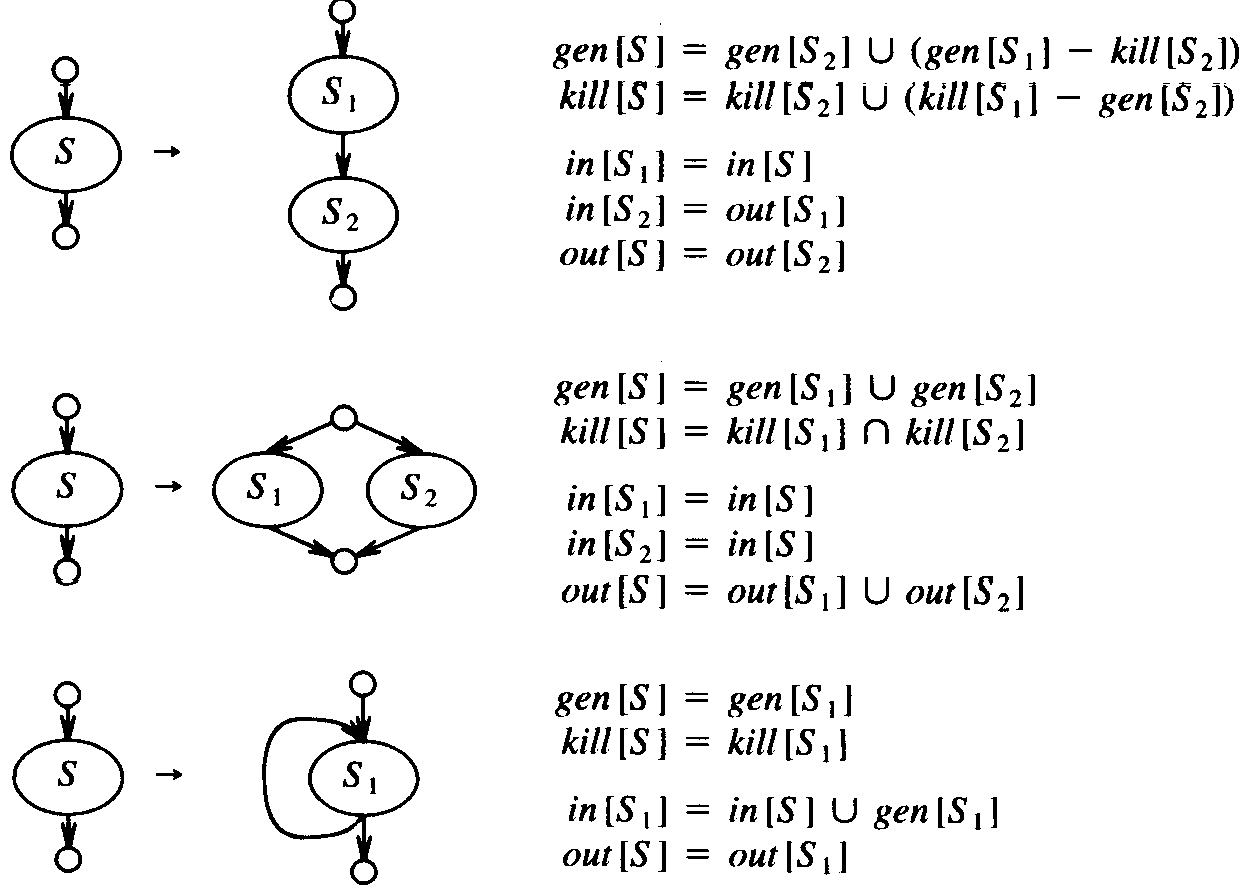
\includegraphics[scale=0.2]{images/bild0-2.png}
    \includegraphics[scale=0.2]{images/b02.epsi}
    \caption{Datenflussgleichungen für zusammengesetzte Anweisungen}
\end{figure}

\begin{figure}[!ht]
    \centering
    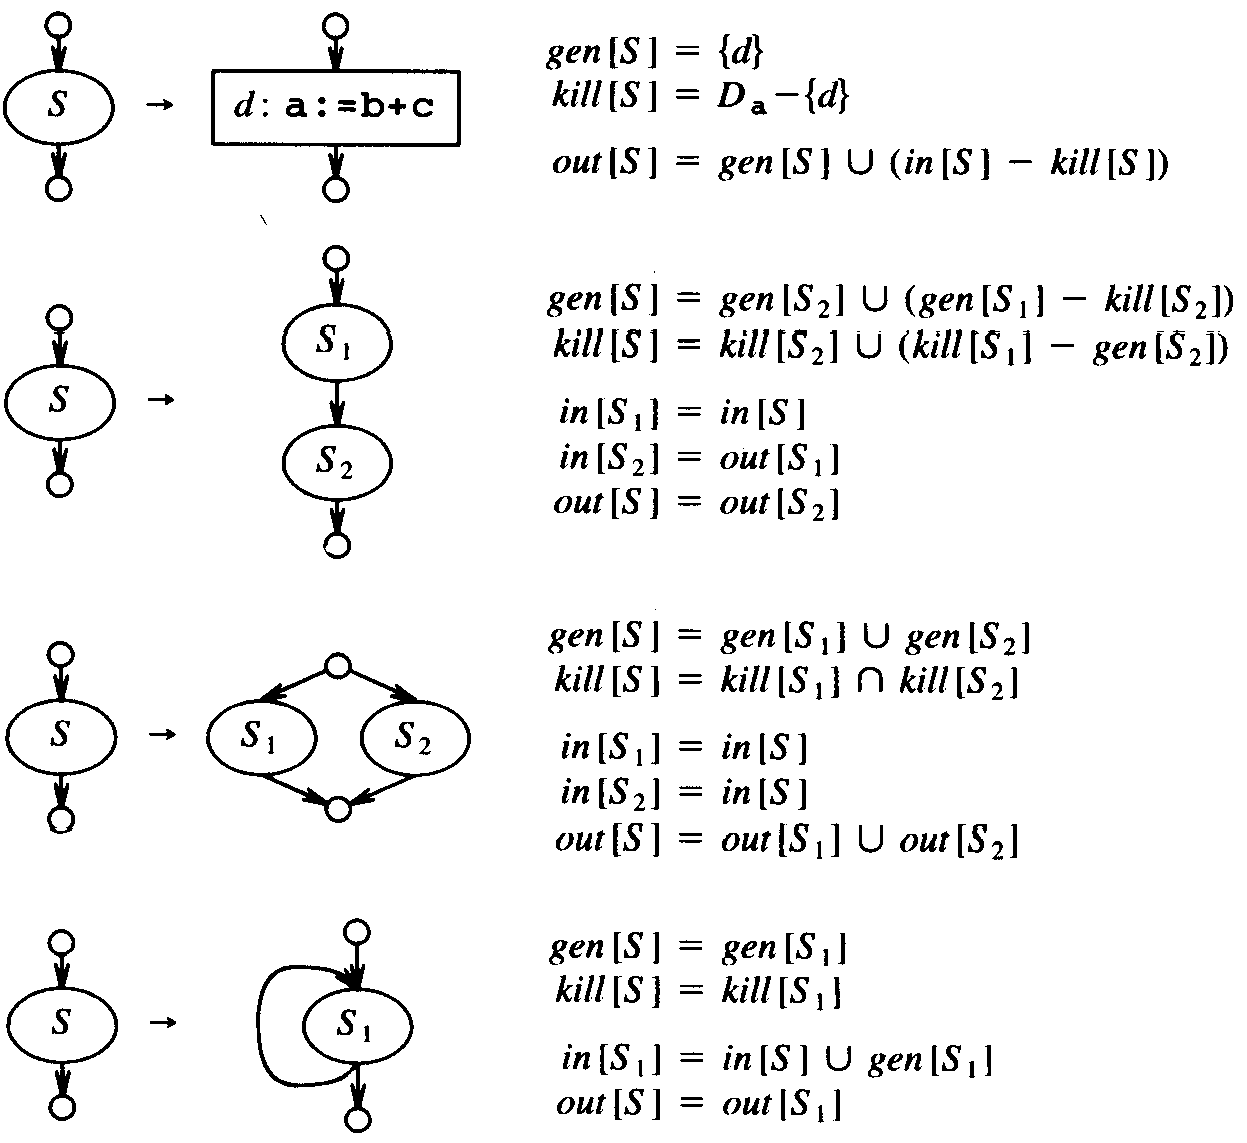
\includegraphics[scale=0.2]{images/bild1-3.png}
    \caption{Datenflussgleichungen für \glqq erreichende Definitionen\grqq\ }
\end{figure}

% subsubsection datenflussgleichungen (end)
\newpage
\subsubsection{Beispielprogramm} % (fold)
\label{ssub:beispielprogramm}
~\\
\begin{figure}[!ht]
    \centering
    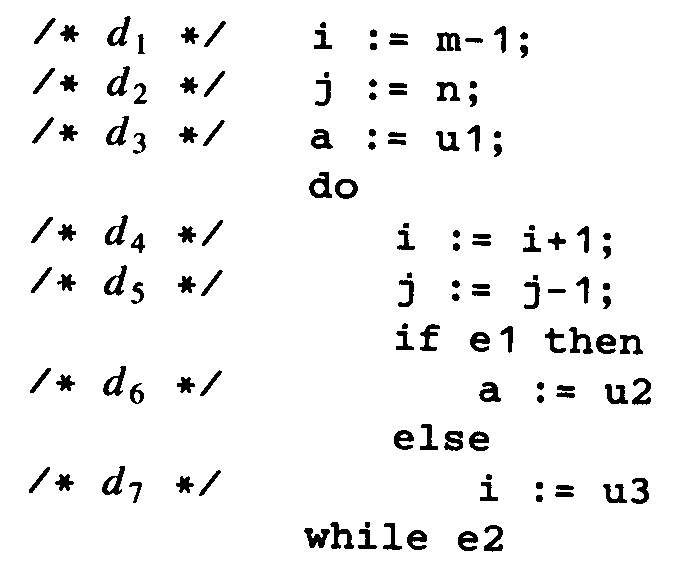
\includegraphics[scale=0.2]{images/bild3-1.png}
    \caption{Beispielprogramm}
\end{figure}
% subsubsection beispielprogramm (end)

\newpage

\subsubsection{Resultat} % (fold)
\label{ssub:resultat}
~\\
\begin{figure}[!ht]
    \centering
    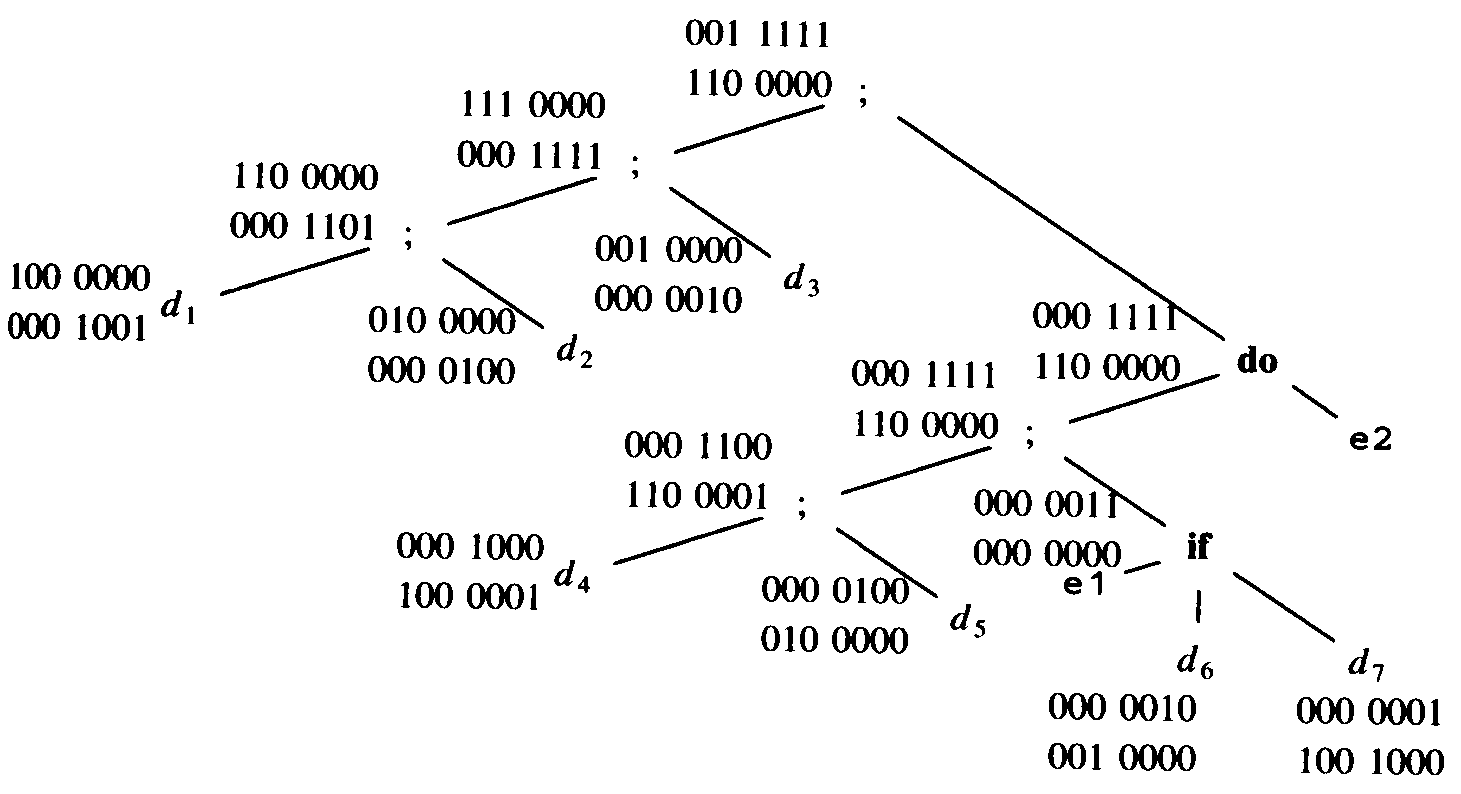
\includegraphics[scale=0.2]{images/bild2-1.png}
    \caption{Resultat}
\end{figure}

% subsubsection resultat (end)

\subsubsection{Nachteile dieses Verfahrens} % (fold)
\label{ssub:nachteile_dieses_verfahrens}
\begin{itemize}
    \item Bitvektor-Darstellung ungeeignet für Arrays
    \item Konflikte, z.\,B. für kill, nur ungenau:
    \begin{itemize}
        \item auf Variablennamen basiert (für Array ungeeignet)
        \item keine Berücksichtigung von eventuell bekannten Schleifengrenzen
        \item keine Berücksichtigung der sequentiellen Ausführungsordnung
    \end{itemize}
    \item für jedes Analyseziel ein neues Datenflussgleichungssystem von Grund auf neu berechnen
    \item im allgemeinen Fall Fixpunktiteration nötig
\end{itemize}
% subsubsection nachteile_dieses_verfahrens (end)
% section konventionelle_abhaengigkeitsanalyse (end)

    % \section{Programm-Modell}
\label{sec:prog-mod}

%Ziel der Vorlesung ist es, Programme automatisch optimal zu
%parallelisieren. Da dieses Problem in dieser Allgemeinheit
%unentscheidbar ist, schränken wir uns wie folgt ein:
\begin{enumerate}
\item Datentypen:
  \begin{enumerate}
  \item Als Datentypen erlauben wir nur (mehrdimensionale) Arrays
    mit beliebigen Einträgen. Beachte: Skalare sind 0-dimensionale
    Arrays.
  \item Lediglich Indizes von Schleifen werden nicht als 0-dimensionale
    Arrays, sondern wirklich als Integers betrachtet.
  \item Darüberhinaus gibt es symbolische Konstanten vom Typ Integer,
    die oft auch als Strukturparameter bezeichnet werden.
  \end{enumerate}
\item Kontrollstrukturen:
  \begin{enumerate}
  \item Das Basiselement ist die Zuweisung an ein Arrayelement.
  \item Die einzige Kontrollstruktur ist die Schleife (beliebig
    verschachtelte Anwendung willkommen).
  \item Als Schleifenunter- bzw. -obergrenzen sind im originalen
    Programm-Modell nur Maxima bzw. Minima affiner Ausdrücke in
    umgebenden Schleifenindizes und in Strukturparametern
    erlaubt; das wird auch der Schwerpunkt der Vorlesung sein,
    wenngleich diese Restriktionen mittlerweile theoretisch aufgelöst
    wurden.
  \end{enumerate}
\item Iterationen:
  \begin{enumerate}
  \item Durch die Schleifen entstehen verschiedene Instanzen von
    Zuweisungen (Operations).
  \item Identifiziert werden Operations durch Angabe des Statements und
    des Iterationsvektors (Vektor, der sich aus den Werten der Indizes der
    umgebenden Schleifenindizes zusammensetzt).
  \item Der Raum aller Operations heißt Index- oder Iterationsraum aller 
    Statements. (Manchmal werden wir die Indexräume von verschiedenen
    Statements auch übereinanderlegen und somit nur einen Indexraum für
    mehrere Statements erhalten, falls die Statements dieselben
    umgebenden Schleifen besitzen.)
  \end{enumerate}
\item Ordnungen:
  \begin{enumerate}
  \item (partielle) Ordnung: reflexiv, transitiv, antisymmetrisch
  \item minimale, maximale Elemente: fehlende Existenz von kleineren,
    größeren Elementen
    % komponentenweise Ordnung
  \item größtes, kleinstes Element: alle anderen sind kleiner, größer
    % Verband der Teilmengenrelation
  \item totale Ordnung: beliebige zwei Elemente vergleichbar
  \item Kette, Antikette: Menge von nur (un-)vergleichbaren Elementen,
    genauer: $A$ Antikette $\Leftrightarrow (\forall x,y \, :\, x,y\in A
    \land x\not= y : \neg ((x\leq y) \lor  (y\leq x)))$
  \item maximale (Anti-) Kette: es gibt keine echte Obermenge, die eine
    \hbox{(Anti-)} Kette ist.
    % maximale Antiketten sind als Mengen partiell geordnet
  \item Theorem 1.1 in \cite{Ban93}.
  \item lexikographische, komponentenweise Ordnung: sollten bekannt sein.
  \end{enumerate}
\item Ausführungsreihenfolge:
  \begin{enumerate}
  \item Für sequentielle Schleifen gilt: In einem perfekt
    verschachtelten Schleifensatz (die Zuweisungen stehen alle in
    demselben Rumpf der innersten Schleife) werden verschiedene
    Instanzen des Schleifenrumpfes gemäß der lexikographischen Ordnung
    der Iterationsvektoren abgearbeitet.
  \item Operation $a$ ist gemäß der sequentiellen Ausführungsordnung
    kleiner als (also vor) Operation $b$, i.Z. $a \prec b$ gdw. ihre
    Iterationsvektoren, eingeschränkt auf gemeinsam umgebende Schleifen,
    lexikographisch kleiner sind, oder diese Vektoren gleich sind und
    $a$ im Programmtext vor $b$ steht.
    %wenn nach dem Entfernen aller gemeinsam umgebenden (äußeren) Schleifen
  \end{enumerate}
\item Abhängigkeiten:
  \begin{enumerate}
  \item geben an, für welche Operations die Ausführungsreihenfolge
    zwingend vorgeschrieben ist. Formale Definition: später.
  \end{enumerate}
\item Graphen
  \begin{enumerate}
  \item (un)gerichtete Graphen: Knoten, Bögen/Kanten (mit/ohne Richtung)
    (Anm: wir verwenden ``Kanten'' auch im gerichteten)
  \item Wege, Pfade: klar; Pfad beachtet die Richtung
  \item Zyklen, Schleifen: Weg, Pfad mit Anfang = Ende
  \item schwach zusammenhängend: ungeachtet der Richtung
  \item stark zusammenhängend: mit Beachtung der Richtung von jedem zu
    jedem
  \item $n$-fach zusammenhängend: nach dem Löschen von $n\!-\!1$ beliebigen
    Kanten immer noch zusammenhängend
  \item schwache, starke Zusammenhangskomponenten: Teilgraphen, die
    schwach, stark zusammenhängend sind
  \item azyklische Kondensation: pro starke Zusammenhangskomponente ein
    Knoten; die ``schwachen Kanten'' übernehmen
  \end{enumerate}
\item Abhängigkeitsgraphen:
  \begin{enumerate}
  \item Iterationsabhängigkeitsgraph: je Operation (oder für jeweils
    übereinandergelegte Operationen) ein Knoten mit Abhängigkeiten als
    Kanten; sehr genau, aber u.U. unbeschränkt.
  \item Statementabhängigkeitsgraph: nur je Statement ein Knoten;
    kleiner, aber ungenauer.
  \end{enumerate}
\item Parallelisierung
  \begin{enumerate}
  \item wirklich notwendige Ordnung von den Abhängigkeiten vorgeschrieben
  \item paralleles Programm (Herleitung später)
  \end{enumerate}
\end{enumerate}




% done (Fabian, 2017-06-29)
    %\setcounter{section}{1}
\section{Polyedermodell}
\label{sec:polymod}


\subsection{Das ursprüngliche Modell}
\label{sec:orig-mod}

\begin{enumerate}
\item Restriktionen:
\begin{enumerate}
\item perfekt verschachtelt
\item Schleifengrenzen: affine Ausdrücke in Strukturparametern und umgebenden
  Indizes und Maxima bzw. Minima davon (für Unter- bzw. Obergrenzen)
\item Arrayindizes affin in den Schleifenindizes und Strukturparametern
\item uniforme Abhängigkeiten
\item ein Schedule und eine Allokation für den kompletten Rumpf;
  Schedule zunächst eindimensional
%\item Schedule und Allokation linear, voneinander lin. unabhängig,
%  gemeinsam volle Dinensionalität
\end{enumerate}
%
\item Modell:
\begin{enumerate}
\item $n$-dimensionaler Schleifensatz im $n$-dimensionalen Raum (je
  Schleife eine Dimension)
\item jeder affine Ausdruck in den Schleifengrenzen definiert einen
  Halbraum
\item Polyeder: der Durchschnitt endlich vieler Halbräume
\item Polytop: beschränktes Polyeder 
\item (Quell-)Indexraum ist ein Polytop
\item Abhängigkeiten durch Pfeile im Indexraum repräsentiert
\item Quellpolytop beinhaltet alle nötigen Informationen
\end{enumerate}
%
\item Raum-Zeit-Abbildung:
\begin{enumerate}
\item Schedule: Funktion, die jeder Operation einen (logischen)
  Ausführungszeitpunkt zuordnet, und dabei die durch die Abhängigkeiten
  vorgegebenen Bedingungen berücksichtigt
\item für das Modell: affine Funktion
\item graphische Bestimmung s. Beispiel der Vorlesung
\item mathematische Bestimmung: lineare Programmierung. Aufgabe:
  minimiere die affine Funktion unter der Nebenbedingung, daß ihr Wert
  für einen abhängigen Punkt größer ist als ihr Wert an dem Punkt, von
  dem er abhängt.
\item Allokation: Funktion, die jeder Operation einen (virtuellen)
  Prozessor zur Ausführung zuordnet
\item für das Modell: affine Funktion, die zum Schedule linear
  unabhängig ist (wegen der realen Maschinen und wegen des Modells
  nötig!)
\item Raum-Zeit-Abbildung: die (mehrdimensionale) affine Abbildung,
  repräsentiert durch die Transformationsmatrix, die sich aus Schedule
  und Allokation zusammensetzt, und so jeder Operation einen
  Raum-Zeit-Punkt der Ausführung zuweist. Zusätzliche Restriktion an die 
  Allokation: die Raum-Zeit-Matrix muß unimodular sein (Determinante
  betragsmäßig 1)
\end{enumerate}
%
\item Transformation des Modells:
\begin{enumerate}
\item Problem: jede einzelne Dimension kann teilweise in Raum und
  teilweise in der Zeit sein
\item Ziel: Separation -- jede Dimension entweder im Raum oder in der Zeit
\item Weg: Basiswechsel = Anwendung der Raum-Zeit-Abbildung auf den
  Quell-Indexraum
\item Resultat: ``verzerrtes'' Polytop: Zielpolytop
\end{enumerate}
%
\item Zurück zum Programm:
\begin{enumerate}
\item Aufgabe: ``scanning'' der Punkte des Zielpolytops
\item parallele Schleifen für die Raumdimensionen und sequentielle
  Schleifen für die Zeitdimensionen
\item Weg: im Quell-Ungleichungssystem die Indizes durch
  ``$T^{-1}*$Zielindizes'' ersetzen und auflösen
\item abhängig von der gewünschten Reihenfolge der Zieldimensionen:
  (a)synchrones Programm
\item Quellindizes durch ``$T^{-1}*$Zielindizes'' ersetzen
\end{enumerate}
\end{enumerate}

\subsection{Das erweiterte Modell}
\label{sec:new-mod}

Erweiterungen:
\begin{enumerate}
\item affine Abhängigkeiten\\[-7mm]
\item stückweise affine Schedules\\[-7mm]
\item per-Statement-Schedule\\[-7mm]
\item nicht-perfekte Verschachtelung\\[-7mm]
\item nicht-unimodulare Raum-Zeit-Abbildungen\\[-7mm]
\item beliebige (z.B. nicht-invertierbare) Raum-Zeit-Abbildungen\\[-7mm]
\item beliebige Schleifentypen\\[-7mm]
\item allgemeine Array-Indizes\\[-7mm]
\end{enumerate}
% done (Fabian, 2017-06-29)
    % \setcounter{section}{2}
\section{Mathematische Grundlagen}
\label{sec:math:i}

\begin{enumerate}
\item unimodulare Abbildungen 
  \begin{enumerate}
  \item ganzzahlig; Determinante=$\pm$1; Inverses ganzzahlig
  \item Bilder von Polytopen unter unimodularen Abbildungen
  \item elementare Zeilentransformationen sind unimodulare Abbildungen:
    \begin{enumerate}
    \item Reversal: Multiplikation einer Zeile mit -1 (!)
    \item Interchange: Vertauschen zweier Zeilen
    \item Skewing: ein Vielfaches einer Zeile zu einer anderen addieren
    \end{enumerate}
  \item Unimodularität abgeschlossen unter Multiplikation
  \item Wesentliches Verfahren: Zeilen-Stufen-Reduktion (Echelon
    Reduktion) einer Matrix $A$ durch eine unimodulare Transformation
    $U$: $U*A = S$
  \item Möglichkeit: Diagonalisierung durch anschließende elementare
    Spaltenoperationen $V$: $S*V = D$
%  \item keine Permutationsmatrizen
  \end{enumerate}
\item ganzzahlig-lineare Gleichungssysteme
  \begin{enumerate}
  \item ``normale'' Gauß-Elimination liefert alle rationalen Lösungen
  \item Einsetzen der frei wählbaren Variablen führt i.A. zu Brüchen in
    den nicht frei wählbaren Variablen
  \item Nachbearbeitung der freien Variablen ist möglich (um
    ganzzahlige Lösungen zu erhalten). Frage: gibt es eine direktere
    Berechnung?  
  \item Bekannt: eine ganzzahlig-lineare Gleichung ist lösbar gdw. der
    ggT $g$ der Koeffizienten $a$ die rechte Seite $c$ teilt
  \item ggT$(a)$ steht in der Zeilen-Stufen-Form des Spaltenvektors
    $(a)$ oben; erste Zeile von $U$ liefert die Multiplikatoren für $a$
  \item Idee: ggT-Restriktion als erstes einsetzen um die Brüche zu
    vermeiden, die bei der Rückwärtssubstitution \`a la Gauß bei der
    letzten Substitution entstehen. Löungsmöglichkeiten:
    Spalten-Stufen-Form (ungewohnt) oder ``transponierte
    Darstellung''. Daher ab sofort:
  \item Variablenvektor $x$ von links multiplizieren (damit Matrizen
    transponiert) und Zeilen-Stufen-Transfor\-mation.  Also: $x*A =
    c$. Dann gilt für eine einzelne Gleichung $x*a=c$ nach unimodularer
    Zeilen-Stufen-Transforma\-tion des Spaltenvektors $a$:
  \item Menge aller Lösungen: $(x_1,\cdots,x_m) = (c/g,t_2,\cdots,t_m)*
    U$
  \item Verallgemeinerung: $x*A = c$ lösbar gdw. $\exists t: t*S =
    c$. Menge aller Lösungen: $x = t*U$.
%  \item keine 2 Variables mit \psi_- und \psi_+
  \end{enumerate}

% sd: Beispiel
\textbf{Beispiel}\\
Ziel: Eine ganzzahlige Lösung ist gewünscht \\
Erinnerung: $U*A = S$ und $x = t*U$

Gleichungssystem:

\begin{align*}
 4x_1 +  6x_2        &= 8 \\
15x_1 + 21x_2 + 6x_3 &= 9
\end{align*}

Lösung nach Algorithmus:

$\left( 
\begin{array}{cc|ccc}
4 & 15 & 1 & 0 & 0\\ 
6 & 21 & 0 & 1 & 0\\ 
0 & 6  & 0 & 0 & 1%
\end{array}%
\right) \leadsto \left( 
\begin{array}{cc|ccc}
2 & 6 & -1 &  1 & 0\\ 
0 & 3 &  3 & -2 & 0\\ 
0 & 0 & -6 &  4 & 1%
\end{array}%
\right) $

Somit:

$\left(
t_1, t_2, t_3
\right) *
\left(
\begin{array}{cc}
2 & 6 \\
0 & 3 \\
0 & 0%
\end{array}
\right)
= 
\left(
\begin{array}{cc}
8 & 9
\end{array}
\right)$

$\Rightarrow t_1 = 4$, $t_2 = \frac{(9-6*4)}{3} = -5$, $t_3 \in \mathbb{Z}$


$\left(
\begin{array}{c|cc}
4 & 1 & 0\\
6 & 0 & 1%
\end{array}
\right) \leadsto \left(
\begin{array}{c|cc}
2 & -1 & 1\\
0 &  3 & -2%
\end{array}
\right)
$
\\
\\Damit ergibt sich als ggT die 2 und als Lösung des Ursprungssystems:

$x = (x_1, x_2, x_3) = t * U = 
\\
(4,-5,t_3) *
\left(
\begin{array}{ccc}
-1 & 1 & 0 \\
3 & -2 & 0 \\
-6 & 4 & 1
\end{array}
\right)
=
(-19-6t_3, 14+4t_3, t_3)
$

% /sd
\item lineare Ungleichungssysteme und Fourier-Elimination
  sukzessive Elimination der einzelnen Variablen: sei $x_j$ die zu
  eliminierende Variable
  \begin{enumerate} 
  \item sortiere die Ungleichungen in untere Schranken für $x_j$, obere
    Schranken für $x_j$ und Ungleichungen, die $x_j$ nicht beinhalten
  \item normiere die beschränkenden Ungleichungen (Koeffizienten der
    zu eliminierenden Variablen alle gleich eins)
  \item lösche die $x_j$ beschränkenden Ungleichungen und füge
    stattdessen die Paare aller möglichen Ungleichungskombinationen ein, 
    die sich ergibt, wenn man alle Unterschranken von $x_j$ allen
    Oberschranken von $x_j$ gegenüberstellt
  \item das resultierende System hat u.U. wesentlich mehr Ungleichungen, 
    aber eine Variable weniger; also: eliminiere nächste Variable
  \item erfolgreiche Termination: keine Ungleichung oder keine Variable
    geblieben (keine Ungleichung = unbeschränkte Variable)
  \item erfolglose Termination: die letzte Ungleichung (ohne
    Variable!!) ist nicht erfüllt
  \end{enumerate}

\textbf{Beispiel}\\
Lösung mit Fourier-Motskin-Algorithmus:
\begin{align*}
0 &\leq t-p\\
t-p &\leq n\\
p &\geq 0\\
p &\leq t-p+2
\end{align*}

\newpage

Somit:
\begin{enumerate}
    \item innerste Schleife\\
$\left.
    \begin{array}{ccc}
        p    &\leq t &\leq n+p \\
        2p-2 &\leq t &\leq n+p
    \end{array}
\right\}$ t unabhängig; Schleifenrumpf:
\begin{procedure}[ht]
\For{$(t=\lceil max(p,2p-2) \rceil ; t \leq \lfloor min(n+p,n+p) \rfloor ; t++)$}{}
\end{procedure}


    \item t eliminiert\\
$\left.
0 \leq p \leq n+2
\right\}$ erweiterter Schleifenrumpf:
\begin{procedure}[ht]
\For{$(p=0; p \leq n+2; p++)$} {
    \For{$(t=\lceil max(p,2p-2) \rceil ; t \leq \lfloor min(n+p,n+p) \rfloor ; t++)$}{}
}
\end{procedure}

    \item p eliminiert\\
$\left. 0 \leq n+2 \right\}$ lösbar, aber nur im Rationalen.
\end{enumerate}


\item affine anstatt linearer Transformationen:
  \begin{enumerate}
    \item Strukturparameter werden wie zusätzliche Variablen behandelt,
      die ``zufällig'' nur einen einzigen Wert zur Laufzeit annehmen.

      Um sicherzustellen, daß sich ihr Wert nicht ändert, werden in den
      Transformationsmatrizen Zeilen eingefügt, die jeden
      Strukturparameter auf sich selbst abbilden.
    \item Eine additive Konstante wird wie ein zusätzlicher
      Strukturparameter behandelt, der zufällig nur den Wert 1 annimmt.
    \item Mathematischer Hintergrund: homogene Koordinaten.
      
      Der Vektor $(x_1,\cdots,x_n,\lambda)$ in homogenen Koordinaten
      entspricht für $\lambda\not=0$ dem Vektor $({x_1\over
        \lambda},\cdots,{x_n\over \lambda})$ in den üblichen
      kartesischen Koordinaten. Für $\lambda=0$ entspricht der Vektor
      $(x_1,\cdots,x_n,\lambda)$ einem Punkt im Unendlichen in Richtung
      $(x_1,\cdots,x_n)$.
  \end{enumerate}
\end{enumerate}
 % done (Niko, 2017-06-29)
    % \setcounter{section}{3}
\section{Abhängigkeitsanalyse im Überblick}


\subsection{Abhängigkeiten im allgemeinen}

Abhängigkeiten in einem Programm spiegeln die durch das Programm
zwingend vorgeschriebene Ausführungsreihenfolge von \emph{Instanzen von
Anweisungen} wider. In imperativen Programmen erfolgt ihre Berechnung
üblicherweise durch die Ermittlung von Speicherstellen, auf die mehrfach
zugegriffen wird. 


\paragraph{Bedingungen}

Eine Operation $o_t$ ist abhängig von einer Operation $o_s$, gdw.
folgende Bedingungen erfüllt sind:
\begin{enumerate}
\item $o_s$ und $o_t$ müssen auf dieselbe
  Speicherzelle zugreifen (\emph{Speicherkonflikt}).
\item $o_s$ und $o_t$ müssen beide durch
  das Programm wirklich generiert werden (\emph{Existenz}).
\item $o_s$ wird gem. der sequentiellen Ausführungsreihenfolge vor $o_t$ 
  ausgeführt---es kann nur eine später ausgeführte Instanz von einer früher
  ausgeführten Instanz abhängig sein (\emph{Ordnung}).
\item Zwischen den zwei Instanzen wird der Wert der Speicherzelle nicht
  mehr modifiziert, d.h., es besteht eine ``direkte Abhängigkeit''
  (\emph{Optimierung}).
\item Mindestens einer der in Konflikt stehenden Zugriffe muß schreibend
  sein (\emph{Bernsteinzusatz}).
\end{enumerate}

\paragraph{Bemerkungen:} Die Optimierung wird bei der praktischen
Berechnung oft vernachlässigt. 

%\paragraph{Bemerkung:} 
Die Bernstein-Bedingungen werden i.a. explizit angegeben (3 Fälle) und
beinhalten Ordnung, Existenz und Speicherkonflikt implizit. Je nach
Analyse-Methode wird die Zusatzbedingung von Bernstein implizit bei der
Auswahl der zu betrachtenden Zugriffspaare berücksichtigt.


\subsection{Abhängigkeiten in Schleifenprogrammen}

Die Abhängigkeits-Analysetechniken sind für verschachtelte
Schleifenprogramme mit Arrays als einziger Datenstruktur relativ gut
entwickelt (Skalar-Variable können dabei als null-dimensionale Arrays
interpretiert werden). 

\noindent
Damit ergibt sich:

\begin{enumerate}
\item Instanzen von Anweisungen sind durch die Anweisung selbst und den
  zugehörigen Iterationsvektor (Vektor der Werte aller umgebenden
  Schleifenindizes) eindeutig charakterisiert.
\item Der Indexraum einer Anweisung ist die Menge aller durch das
  Schleifenprogramm aufgezählten Indexvektoren für diese Anweisung.
\item Die sequentielle Ausführungsreihenfolge von zwei Instanzen ist
  gegeben durch die lexikographische Ordnung auf dem gemeinsamen Präfix
  ihrer Iterationsvektoren und---bei deren Gleichheit---durch die
  textuelle Reihenfolge der Anweisungen im Programmtext.
\item Speicherkonflikt liegt genau dann vor, wenn zwei Instanzen auf
  dasselbe Array zugreifen und für jede Array-Dimension auch denselben
  Index liefern. ACHTUNG: Nicht die Schleifen-Indizes, sondern die
  Array-Indizes nach dem Einsetzen der Schleifen-Indizes
  (=Iterationsvektoren) müssen übereinstimmen.
\end{enumerate}

\paragraph{Beispiel:} 3 Schleifen, 2-dim. Arrays.

\paragraph{Begriffe:}

\begin{enumerate}
\item Die Abhängigkeit geht von der \emph{Quelle} zum \emph{Ziel}.
\item Im Fall von perfekt verschachtelten Schleifen ist der
  \emph{Abhängigkeitsvektor} (oder \emph{Distanzvektor}) ist die Differenz: Ziel-Iterationsvektor minus
  Quell-Iterationsvektor. Er ist also immer lexikographisch nicht-negativ (also hinsichtlich des zeitlichen Ablaufs).
\item Eine Abhängigkeit heißt \emph{uniform}, wenn der Abhängigkeitsvektor an
  jedem Punkt des Indexraumes identisch ist.
\item Durch \emph{Richtungsvektoren}, in denen die Werte der
  Abhängigkeitsvektoren durch ihr Signum ersetzt werden, kann man selbst
  nicht-uniforme Abhängigkeiten (zu Lasten der Genauigkeit) effizient
  darstellen. 
\item Eine Abhängigkeit wird von derjenigen Verschachtelungstiefe
  \emph{getragen}, deren erster Eintrag im Richtungsvektor größer als
  null ist. Ist der Richtungsvektor gleich dem Nullvektor, so heißt die
  Abhängigket \emph{schleifenunabhängig}.
\end{enumerate}


Je nachdem, ob das Ziel oder die Quelle ein lesender oder ein
schreibender Zugriff ist, werden verschiedene \emph{Typen} von
Abhängigkeiten unterschieden: 

\smallskip

\begin{center}
\begin{tabular}{||r|cc||}
\hline
Ziel & \multicolumn{2}{|c||}{Quelle}\\
 & liest & schreibt \\
\hline
liest & input & true\\
schreibt & anti & output\\
\hline
\end{tabular}
\end{center}

\paragraph{Bemerkungen:} 

\begin{enumerate}
\item I.A. werden input dependences wegen der Bernstein-Zusatzbedinung
  vernachlässigt.
\item True dependences, die das Optimierungskriterium erfüllen, heißen
  auch flow dependences. (ACHTUNG: Diese Begriffe werden in der Literatur
  uneinheitlich verwendet.)
\end{enumerate}

\paragraph{Graphische Darstellung:}

Die graphische Darstellung erfolgt entweder durch den
\emph{Iterations-Abhängigkeitsgraphen} oder den
\emph{Statement-Abhängigkeitsgraphen}.
 % done (Fabian, 2017-06-29)
    % \setcounter{section}{4}
\section{Abhängigkeitsanalyse nach Banerjee}

\subsection{Normalisierung des Schleifenkopfes}

Die Behandlung von Schrittweiten ungleich von eins, insbesondere von
negativen Schrittweiten, macht die Abhängigkeitsanalyse aufwendig. Daher
normalisiert man Schleifen oft wie folgt:



  % {\sf for $i:=x$ to $y$ step $s$ do $R(i)$}
 
\begin{minipage}{.4\textwidth}
  \begin{algorithm}[H]
      \SetKw{KwStep}{step}
      \For{$i:=x$ \KwTo $y$ \KwStep s}{
        \( R(i) \)
      }
  \end{algorithm}
\end{minipage}
\begin{minipage}{.5\textwidth}
    \qquad $\to$ \qquad  
    \begin{algorithm}[H]
          \SetKw{KwStep}{step}
          \For{\( i' := 0\) \KwTo \( \frac{y\!-\!x}{s} \) \KwStep 1}{
            \( R(i' \cdot s + x) \)
          }
      \end{algorithm}  
\end{minipage}
  % {\sf for $i':=0$ to ${y\!-\!x}\over s$ step $1$ do $R(i'*s+x)$}  
  ~\\
(vgl. \cite{Zima90}, S. 175)

\subsection{Konflikt-Gleichungssystem}

Zwei Operations $o_s$ und $o_t$ müssen auf dieselbe Speicherzelle
zugreifen, d.h., die Variablennamen und die Array-Indizes, die $o_s$ und
$o_t$ ansprechen, müssen in allen Komponenten übereinstimmen. Für die
entsprechenden Iterationsvektoren $i_s$ und $i_t$ muß also in
Matrixnotation gelten: 
$$i_s * A + a_0 = i_t * B + b_0,$$ wobei jede Spalte von $A$ ($B$) die
Koeffizienten eines Array-indexes beinhaltet und $a_0$ ($b_0$) den
konstanten Anteil bechreibt \cite{Ban93}.

Anders notiert: $$(i_s, i_t) * \left( {A \atop -B} \right) = b_0-a_0$$

Lösung wie im Abschnitt für mathematische Grundlagen
beschrieben. 

\subsection{Existenz-Ungleichungssystem}

Die zwei Operations $o_s$ und $o_t$ müssen beide durch das Programm
wirklich generiert werden, d.h., die Iterationsvektoren $i_s$ und $i_t$
müssen im jeweiligen Indexraum der entsprechenden Statements
sein. Matrixnotation: $$p_0 \leq i * P \hbox{\qquad bzw. \qquad} i*Q \leq
q_0$$ für die unteren bzw. oberen Grenzen der Indexräume. Diese
Ungleichungen müssen natürlich sowohl für $i_s$ als auch für $i_t$
aufgestellt werden.

Die -- ggfs. parametrisierten -- Lösungen des Konflikt-Gleichungssystems
kann man in das Ungleichungssystem einsetzen und so die Lösbarkeit
innerhalb des Indexraums überprüfen, bzw. ggfs. die Wahl der Parameter
einschränken.

\subsection{Ordnungsrelation und Abhängigkeitstypen}

Bis hierher haben wir zwei Operations $o_1$ und $o_2$, die eine
Abhängigkeit verursachen. Frage: Wer ist Quelle, wer Ziel?  Wir wissen:
Operation $o_s$ muß gem.  der sequentiellen Ausführungsreihenfolge vor
$o_t$ ausgeführt werden. Lösung: teile die (ggfs. parametrisierten)
Paare von Iterationsvektoren so in zwei Mengen ein, daß in einer stets
gilt $o_1 \prec o_2$ und in der anderen $o_2 \prec o_1$ (ggfs. unter
Aufteilung der Räume für die Wahl der Parameter). Dadurch sind jeweils
Quelle und Ziel identifiziert, was damit auch die Typen der
Abhängigkeiten lt. Tabelle im vorigen Abschnitt festlegt. (Die Ordnung ist bei dem Verfahren nach Banerjee nicht a priori bekannt.)

\subsection{Optimierung}
Die Optimierung wird bei Banerjee komplett vernachlässigt.

\subsection{Randbemerkung: Sonderfälle}
Banerjee stellt Sonderfälle vor, in denen sich die Analyse etwas vereinfacht.
\begin{enumerate}
\item ``regulärer'' Schleifensatz: perfekt, $P=Q$ und $A=B$, dann für $d
  = i_s-i_t$. Dadurch $$ d * A = a_0-b_0 \hbox{\qquad und \qquad} p_0-q_0 \leq
  d*P \leq q_0-p_0$$. Die Halbierung der Variablenzahl macht das
  Gleichungssystem einfacher und die Ordnung handlicher.
\item ``rechteckiger'' Schleifensatz: $P=Q=I_m$ (Identität) und $A$ und
  $B$ in Diagonalform (aber nicht unbeding identisch). Dadurch
  unabhängige $m$ Gleichungen mit je 2 Variablen, die unabhängig
  voneinander aufgelöst werden können. Die Zeilenstufenreduktion wird
  daher etwas übersichtlicher, aber im Endeffekt keine spürbare
  Erleichterung.
\end{enumerate}

% sd
\subsection{Beispiel zur Abhängigkeitsanalyse nach Banerjee}
\textit{Programmcode:}\\

\begin{procedure}
\SetLine
\For{$i=10$ \KwTo $200$}{
    \For{$j=7$ \KwTo $167$}{
        
        \bf{S:} $X[2i+3, 5j-1, j]$ :=...\\
        \bf{T:} ... := ... $X[i-1,2i-6,3j+2]$
    }
}
\end{procedure}
~\\
\textit{Konfliktgleichungssystem:} (gestrichene Var. f. T)\\

\begin{align*}
2i+3 &= i^\prime  - 1\\
5j-1 &= 2i^\prime - 6\\
 j   &= 3j^\prime + 2
\end{align*}

nach Banerjee:\\

$A=
\left(
\begin{array}{ccc}
2 & 0 & 0\\
0 & 5 & 1
\end{array}
\right), a_0 = (3,-1,0)$

$B=
\left(
\begin{array}{ccc}
1 & 2 & 0\\
0 & 0 & 3
\end{array}
\right), b_0 = (-1, -6, 2)$


$(i,j) * A + a_0 = (i^\prime, j^\prime) * B + b_0 \\
\Leftrightarrow
(i,j,i^\prime,j^\prime) * 
\left(
\begin{array}{c}
A\\
-B
\end{array}
\right)
= b_0 - a_0$\\
Eingesetzt:\\
$(i,j,i^\prime,j^\prime) * 
\left(
\begin{array}{ccc}
2 & 0 & 0\\
0 & 5 & 1\\
-1&-2 & 0\\
0 & 0 &-3
\end{array}
\right)
= (-4,-5,2)$

\textit{Lösen}

$\left(
\begin{array}{ccc|cccc}
 2 & 0 & 0 & 1 & 0 & 0 & 0 \\
 0 & 5 & 1 & 0 & 1 & 0 & 0 \\
-1 &-2 & 0 & 0 & 0 & 1 & 0 \\
 0 & 0 &-3 & 0 & 0 & 0 & 1
\end{array}
\right) \leadsto \left(
\begin{array}{ccc|cccc}
-1 &-2 & 0 & 0 & 0 & 1 & 0 \\
 0 & 1 & 1 & 1 & 1 & 2 & 0 \\
 0 & 0 & 1 & 5 & 4 &10 & 1 \\
 0 & 0 & 0 &15 &12 &30 & 4
\end{array}
\right)$


$(t_1,t_2,t_3,t_4) * S = (-4, -5, 2) \\
\Rightarrow t_1 = 4; t_2= 3; t_3 = -1; t_4 \in \mathbb{Z} \\
\Rightarrow (i,j,i^\prime,j^\prime) = (t_1,t_2,t_3,t_4) * U =
(-2+15t_4; -1+12t_4; 30t_4; -1+4t_4)$
somit kann man folgende Abhängigkeiten folgern:\\
$\langle (-2 + 15t_4; -1+12t_4), S \rangle \stackrel{?}{\leftrightarrow}
 \langle (30t_4;-1+4t_4), T \rangle$ für $t_4 \in \mathbb{Z}$ 
~\\
\textit{Existenzungleichungssystem:}\\

$P = Q =
\left(
\begin{array}{cc}
1 & 0 \\
0 & 1
\end{array}
\right), p_0 = (10,7), q_0 = (200,167)$
~\\
\textit{Gleichungen:}\\

$\begin{array}{cc}
\underbrace{
\begin{array}{ccc}
10 &\leq -2+15t_4 &\leq 200 \\
7  &\leq -1+12t_4 &\leq 167
\end{array}
}_{\text{Existenz von} (i,j) \text{bei S}} &
\underbrace{
\begin{array}{ccc}
10 &\leq 30t_4 &\leq 200 \\
 7 &\leq-1+4t_4 &\leq 167
\end{array}
}_{\text{Existenz von} (i,j) \text{in T}}

\end{array}$

$\stackrel{FM}{\leadsto} 2 \leq t_4 \leq 6$
~\\
\textit{Ordnung:} Richtung der Abhängigkeit $\leftarrow$ oder $\rightarrow$ ?\\

Lexikographische Ordnung: $i < i^\prime$ oder $i = i^\prime \land j < j^\prime$\\
\begin{equation}
\begin{split}
i<i^\prime &\Leftrightarrow -2+15t_4 < 30t_4\\
           &\Leftrightarrow    15t_4 > -2\\
           &\Leftrightarrow      t_4 >-\frac{2}{15}
\end{split}
\end{equation}
da $t_4 \geq 2 \Leftrightarrow true$\\
Lösung $\underbrace{\langle (-2 + 15t_4; -1+12t_4), S \rangle}_{\text{schreibt} \Rightarrow \text{true Dependence}} \rightarrow
 \underbrace{\langle (30t_4;-1+4t_4), T \rangle}_{\text{liest}}$ für $2 \leq t_4 \leq 6$\\

Distanzvektoren: \glqq Ziel-Quelle\grqq\\
$(30t_4; -1+4t_4) - (-2+15t_4; -1+12t_4) =\\
(2+15t_4; -8t_4)$ für $2\leq t_4 \leq 6)$.

Richtungsvektor: $(+,-)$\\
Level: 1\\
~\\
\textit{Statement-Abhängigkeits-Graphen:}\\

\entrymodifiers={++[o][F-]}
\xymatrix{
S \ar[d]^{( 2+15t_4; -8t_4 )} \\
T 
}
~\\
\textit{Optimierung:} nicht bei Banerjee.\\
~\\
Somit führt Banerjee zum Abhängigkeitsvektor und gibt alle Abhängigkeiten inklusive einiger eigentlich nutzloser aber für den Algorithmus notwendiger \glqq Initialisierungsabhängigkeiten\grqq\ zurück (Initialisierungsschrott).
 % done (Fabian, 2017-06-29)
    % \section{Datenflußanalyse und \\Single-Assignment-Konversion}
%----------------------------------------------------------------------
Die Datenflußanalyse nach Feautrier \cite{Fea91} ist aufwendiger als die von
Banerjee, berücksichtigt aber auch die Optimierung.

\subsection{Ansatz}
Im Gegensatz zu Banerjee werden nicht alle Abhängigkeiten gesucht,
sondern nur echte Datenflußabhängigkeiten. Daher werden nicht alle
Zugriffspaare untersucht, sondern zu jedem Lesezugriff werden alle
Schreibzugriffe als mögliche Quellen betrachtet. Der Lesezugriff ist
damit die Senke; der Typ der Abhängigkeiten ist \emph{flow}.

Durch diesen Ansatz wird die Existenz des Lesezugriffs zu einer immer
erfüllten Voraussetzung, die für das Konfliktgleichungssystem und die
Existenz der Quelle oder auch die Optimierung zusätzliche Informationen
bedeutet.

Das System aus Konfliktgleichungen, Existenzungleichungen und
Ordnungsungleichungen wird einem Tool zur parametrisierten, ganzzahlig
linearen Optimierung (z.B. PIP) in einem Aufwasch präsentiert.

Die (lokal bereits optimierten) Lösungsergebnisse werden in einem
zweiten Arbeitsgang ``gemischt''.

Resultat: für Polyeder: eindeutige Quellen je Lesezugriff.

\subsection{Single-Assignment-Konversion}
\begin{enumerate}
\item einmalige Zuweisung durch ``Umleiten'' der Schreibzugriffe in
  neue Arrays, die voll indiziert sind.
\item Wiederherstellung der Semantik durch Einsetzen der Quelle in den
  Lesezugriffen.
\end{enumerate}

\subsection{Verfahren von Feautrier:}
Bei Feautrier ist die Ordnung das \emph{Input Kriterium}. Damit sind alle Gleichungen in ein System pro Dimension aufstellbar. (Für die Antiabhängigkeiten (wg. der Inputvernachlässigung) gibt es keine derartige Optimierung, da man nicht überlesen kann.)
\entrymodifiers={++[][]}

\xymatrix{
*+[F]{x = \dots} \ar[d] |{Datenfluss}
          \ar@/^6pc/[ddd]|{Banerjee-Abh.}\\
*+[F]{\dots = x} \ar[d] |{Anti-Abh.} \\
*+[F]{x = \dots} \ar[d] |{Datenfluss}\\
*+[F]{\dots = x}
}

~\\[0.5cm]
\emph{Konfliktgleichungssystem:} gleich Banerjee\\[0.2cm]
\emph{Existenz-Ungleichungen:} Welche \glqq Writes \grqq schreiben den an der aktuellen Stelle gelesenen Wert? Welches \glqq Write \grqq ist das letzte? $\leftarrow$ Optimierung\\[0.2cm]
\emph{Read-Existenz:} Kontext für die Analyse, Feautrier liefert nur optimierten True-Deps., also die Flow-Dependences.\\[0.2cm]
\emph{Folge:} die Ordnung wird Input des Verfahrens:\\
als Ungleichungssysteme (je Fall für die lexikographiesche Ordnung eine)

\subsubsection{Beispiel}
\textit{Programmcode:}

\begin{procedure}[H]
\SetLine
\For{$i=0$ \KwTo $n$}{
    \textbf{R:} $A[0,0] := ...$\\
    \textbf{S:} $X[i]   := A[i,0]$\\
    \For{$j=1$ \KwTo $n$}{
        \For{$k=1$ \KwTo $n$}{
            \textbf{T:} $A[i+k-1,j-1]:=...$\\
        }
    }
}
\end{procedure}

\textit{Frage:} Wer hat den Wert geschrieben, der in $\langle (i),S \rangle$ gelesen wird?\\

\textbf{S-T-Konflikt}\\
\begin{enumerate}
    \item \textit{Instanz:} $\langle (i), S \rangle$, $\langle (i^\prime, j^\prime, k^\prime), T) \rangle$

    \item \textit{Konfliktgleichungssystem:} \\
        $\begin{array}{cc}
        \left.
        \begin{array}{c@= l}
            i & i^\prime + k^\prime-1\\
            0 & j^\prime -1
        \end{array} \right\} & \Leftrightarrow
        \begin{array}{c@= l}
            k^\prime & i-i^\prime +1 \\
            j^\prime & 1
        \end{array}
        \end{array}$


    \item \textit{Existenzungleichungen:} nur für $i^\prime, j^\prime, k^\prime$\\
        \begin{align*}
        0 &\leq i^\prime \leq n \\
        1 &\leq j^\prime \leq n \\
        1 &\leq k^\prime \leq n
        \end{align*}
        Kontext: $0 \leq i \leq n$\\
        (Da hier kein Interesse für Anti-Abhängigkeiten besteht, erfolgt alles im Kontext von i. \glqq Ich bin Statement S, welche Iteration hat geschrieben, was ich gerade lese?\grqq)
    \item \textit{Ordnung:} soll $\langle ( i^\prime, j^\prime, k^\prime), T \rangle \rightarrow \langle (i), S \rangle$\\

    $(i^\prime < i) \lor \underbrace{(i^\prime = i \land \text{T textuell vor S})}_{false}$


$
\begin{array}{cc}
% \begin{array}{cc}
% \left.
\begin{array}{cccccc}
i^\prime & j^\prime & k^\prime & i & n & 1  \\
-1       & 0        & -1       & 1 & 0 & 1  \\
1        & 0        & 1        & -1& 0 & -1 \\
0        & 1        & 0        & 0 & 0 & -1 \\
0        & -1       & 0        & 0 & 0 & 1  \\
% \end{array}\right\} & Konfliktgleichungen\\
% \left.
% \begin{array}{cccccc}
1        & 0        & 0        & 0 & 0 & 0  \\
-1       & 0        & 0        & 0 & 1 & 0  \\
0        & 1        & 0        & 0 & 0 & -1 \\
0        & -1       & 0        & 0 & 1 & 0  \\
0        & 0        & 1        & 0 & 0 & -1 \\
0        & 0        & -1       & 0 & 1 & 0  \\
% \end{array} \right\} & Existenzungleichungen\\
% \left.
% \begin{array}{cccccc}
0        & 0        & 0        & 1 & 0 & 0  \\
0        & 0        & 0        &-1 & 1 & 0  \\
% \end{array} \right\} & Kontext\\
% \left.
% \begin{array}{cccccc}
-1       & 0        & 0        & 1 & 0 &-1
% \end{array} \right\} & Ordnung i^\prime < i\\
\end{array}
& \geq 0
\end{array}$\\

(Die ersten vier Zeilen sind das Konfliktgleichungssystem, dann folgen 6 Zeilen lang das Existenzungleichungssystem, dem sich dann eine Kontextzeile und eine Ordnung (\( i^\prime < i \)) anschließt.)
Lösung des Gleichungssystems mit FM.\\

Zwischenergebnis: \\$\langle (i^\prime, 1, i-i^\prime+1), T \rangle \rightarrow \langle (i), S \rangle *\\$ für $ 0 \leq i^\prime < i \leq n \text{, } 1\leq i-i^\prime + 1 \leq n \\
\text{ für Kontext } 0\leq i \leq n$

\item \textit{Optimierung}\\
    gesucht: letzte (lex. größte) Instanz von T mit *, die vor $\langle (i), S \rangle$ ausgeführt wird. \\
    Lösung: $i^\prime = i-1\\
            \Rightarrow \langle (i-1,1,2), T \rangle \rightarrow \langle (i), S \rangle$ für $i \geq 1$
\end{enumerate}

\textbf{S-R-Konflikt}\\
    \begin{enumerate}
    \item $\langle (i), S \rangle \text{,} \langle(i^\prime), R \rangle$
    \item $0=i \land 0 = 0$
    \item $0 \leq i^\prime \leq n \text{ im Kontext } 0 \leq i \leq n$
    \item $i^\prime < i \lor (i^\prime = i \land \text{ R vor S}) \Leftrightarrow i^\prime \leq i$
    \item $i^\prime = i \\
        \Rightarrow \langle (i),R \rangle \rightarrow \langle (i), S \rangle \text{ für } i=0 \\
        \Rightarrow \langle (0),R \rangle \rightarrow \langle (0), S \rangle$

    \end{enumerate}
Datenfluss: \\
\begin{procedure}
    src($ \langle (i), S \rangle $) =\\ \eIf{$i=0$}{$\langle (0), R \rangle$}{$\langle (i-1,1,2),T \rangle$}
\end{procedure}

Vorsicht: Falls die Bedingungen der Schleifenindizes nicht disjunkt sind, geht die Abhängigkeit von Maximum der Quellen (bzgl. der Ausführungsordnung) aus.

%% --------------------------- CfFada -------------------------------------------------

\subsection{Verfahren via CfFada:}

CfFada heißt ausgeschrieben \glqq Controllflow based Fuzzy array dataflow\grqq.\\
Dieses weiteres Verfahren wird motiviert durch die Existenz von \glqq if-Statements\grqq\ , \glqq unstrukturierte Programme\grqq\ und die erhöhte \glqq Präzision\grqq.\\
\paragraph{Idee:}
\begin{enumerate}
    \item Zusammenführen von
    \begin {enumerate}
        \item traditionellen (universell einsetzbar, ungenau) und
        \item einem Feautrier-ähnlichem Verfahren
    \end{enumerate}
    \item (Effizienz)
\end{enumerate}

\paragraph{Prinzipielles Vorgehen:}
\begin{enumerate}
    \item Konstruiere den Kontrollflußgraphen (CFG)
    \item Für jeden Zugriff a:
        \begin{enumerate}
            \item Annotiere den CFG mit den für a relevanten Relationen - unter Berücksichtigung der umgebenden Prädikate
            \item starte mit leerer Abhängigkeitsmenge (alles bottom) und Ordnungsrelation $(=,...,=)$ bei a. (\( i = i^\prime = \dots \))
            \item durchlaufe den CFG rückwärts
            \item bei Schleifen: durchlaufe die Rückwärtskanten von innen nach außen und passe die aktuell gültige Ordnungsrelation an
            \item bei \glqq conflicting accesses\grqq : mische die neuen und alten Abhängigkeiten unter Berücksichtigung der Optimierung
        \end{enumerate}
\end{enumerate}


\paragraph{Anmerkungen:}

\begin{enumerate}
    \item Implementierung mit Omega (Presburger Arithmetik) \( \rightarrow \) Genauigkeit
    \item unstrukturierte Programme \( \rightarrow \) Abschätzung der Ordnungsrelation
    \item vorzeitiges Analyse-Ende möglich, wenn alle möglichen letzten Quellen gefunden wurden.
    \item Der Hauptunterschied zu Feautrier besteht in der Tatsache, dass CfFada mit if-Statemants umgehen kann.
    \item textuell getragene Abhängigkeiten entspricht sprachlich den Schleifenunabhängigen Abhängigkeiten
    \item Mischen: Schneiden und Optimierung
    \item \( \Box := \) Merge/Mischen
    \item \( W(6) := \) Write-Set von 6
\end{enumerate}


\subsubsection{Beispiel zur Abhängigkeitsanalyse nach CfFada}

\begin{wrapfigure}{r}{0.6\textwidth}
    \begin{flushright}
        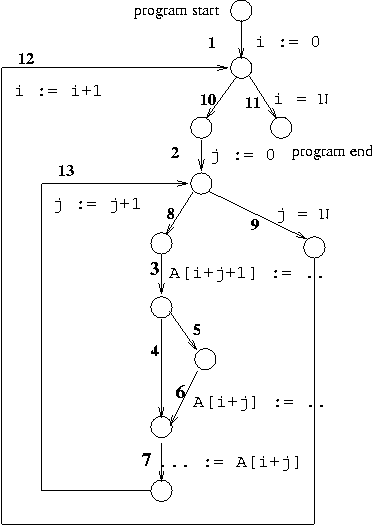
\includegraphics[scale=0.5]{images/cffada.png}
        \caption{Ablaufgraph}
        \vspace{+40pt}
    \end{flushright}

\end{wrapfigure}

\textit{Programmcode:}\\
    \begin{procedure}[H]
    \SetLine
    \For{$i=0$ \KwTo $N$}{
        \For{$j=0$ \KwTo $N$}{

            \bf{3:} $A[i+j+1]$ = ... \\
            \eIf{$P$}
                {\bf{6:} $A[i+j]$ = ...\\}{}
            \bf{7:} ... = $A[i+j]$

        }
    }
    \end{procedure}

~\\[6cm]
\textbf{Kontext}\\
Read-Statement 7\\
Operationen: $\langle (i,j), 7 \rangle$ für $0 \leq i, j \leq N$\\
\\
\textbf{Annotierung}\\
Statement 3\\
Operationen: \(\langle (i^\prime,j^\prime), 3 \rangle\) für \( \underbrace{0 \leq i^\prime, j^\prime \leq N}_{Existenz} \land \underbrace{i^\prime + j^\prime + 1 = i + j}_{Konflikt}\)\\
Statement 6\\
Operationen: \dots\\

\textbf{Durchlauf}\\
\begin{enumerate}
    \item {Ordnung: \(i=i^\prime \land j=j^\prime\) \\
        \(src^{(0)} = {\perp}\)\\
        \begin{enumerate}
            \item Start: 7
            \item die 4 hoch: (Kante mit Label 4)\\
                  Keine neuen Quellen\\
                  \(scr_{4}^{(1)} = \lbrace \perp \rbrace\)
            \item die 6 hoch: (überprüfe Existenzun- und Konfliktgleichungen)\\
                  \(src_{6}^{(1)} = src^{(0)} \Box W(6) = \)
    \(\begin{cases}  \langle (i,j), 6 \rangle , & \mbox{ für } P^\prime(i,j) \\
                     \perp ,                    & \mbox{ sonst }
    \end{cases}  \)

            \item bei n1 Mischen:\\
                \(scr_{n1}^{(1)} =
    \begin{cases} \langle (i,j),6 \rangle, & \mbox{ für } p^\prime(i,j) \\
                  \perp,                   & \mbox{ sonst }
                \end{cases} \)

            \item die 3 hoch:\\
                  Keine neuen Quellen, da die aktuelle Ordnung $\lightning$ Konfliktgleichung. (Wäre P immer true, könnte man an n1 abbrechen.)
            \item die 13 hoch \(\Rightarrow\)

        \end{enumerate}
        }
    \item {Ordnung: \(i=i^\prime \land j^\prime < j\) \\
      \begin{enumerate}
         \item die Kanten 7, 4 bringen nichts neues.
         \item die 6 hoch: \\
           Keine neuen Quellen, da die aktuelle Ordnung $\lightning$ Konfliktgleichung.
         \item n1: nichts neues zu mischen \(\Rightarrow\) alles bleibt
         \item die 3 hoch: \\
           \(src^{(2)} = src^{(1)} \Box W(3) = \) \\ \( =
           \begin{cases} \langle ( i^\prime, j^\prime), 3) \rangle, & \mbox{ für } i^\prime + j^\prime + 1 = i + j \land \neg P^\prime(i,j) \land 0 \leq i^\prime \leq N \land 0 \leq j^\prime \leq N \\ & \mbox{ mit aktueller Ordnung}\\
             \langle (i,j),6 \rangle , & \mbox{ für } P^\prime(i,j) \\
             \perp, & \mbox{sonst}
           \end{cases}
\)
           \\ \(\stackrel{j^\prime+1=j}{=}
           \begin{cases}
             \langle ( i, j-1), 3 \rangle, & \mbox{ für }\neg P^\prime(i,j) \land j > 0 \land 0 \leq j-1 \leq N \\
             \langle (i,j),6 \rangle , & \mbox{ für } P (i,j) \\
             \perp , & \mbox{ sonst, d.\,h. } j = 0 \land \neg P(i,0)
           \end{cases}
           \)
         \item Kante 8: -
         \item Kante 2: -
         \item Kante 10: -
         \item Kante 12: -
      \end{enumerate}
      }

      \item {Ordnung: \(i^\prime < i, j^\prime\) beliebig
          \begin{enumerate}
            \item Kante 9,13,7,4: -
            \item Kante 6: \\
              wegen Optimierung: \(j= 0 \land \neg P^\prime (i,j)\) \\
              Ordnung: \(i^\prime < i \) \\
              Konflikt: \( i^\prime + j^\prime = i + 0 \) \\
              Existenz: \( P^\prime(i^\prime, j^\prime) \) \\
              neue Quellen: \( \langle ( i^\prime, i-i^\prime ), 6 \rangle \text{ für } j=0, i^\prime < i , P(i^\prime, i - i ^\prime) \land \neg P(T, i-T) \text{ für } i^\prime < T \leq i \) \\

\( src^{(3)}_{n1} =
\begin{cases}
  \langle (i,j), 6 \rangle, & \mbox{ für } P(i,j) \\
  \langle (i,j-1), 3 \rangle, & \mbox{ für } j \geq 1 \land \neg P (i,j) \\
  \langle (i^\prime, i-i^\prime),6 \rangle, & \mbox{ für } j=0 \land i^\prime < i \land P(i^\prime, i - i^\prime) \land \neg P(T,i-T) \\ & \mbox{ für } i^\prime < T \leq i \land i^\prime \geq 0 \land i \geq 1 \\
  \perp, & \mbox{ für } j=0 \land \neg P(i^\prime, i - i^\prime) \text{ für alle } 0 \leq i^\prime \leq i
\end{cases} \)

\item Kante 3:\\
  wegen Optimierung: \( i^\prime = i - 1, j=0 \stackrel{Konfl. Gl.}{\Rightarrow} j^\prime = 0\) \\
  neue Quelle: \( \langle (i-1,0), 3 \rangle \text{für} j=0 \land i \geq 1 \land \neg P(i,0) \land \neg P(i-1,1) \) \\
\( \Rightarrow src =
\begin{cases}
  \langle (i, j), 6 \rangle, & \mbox{für } P(i,j) \\
  \langle (i, j-1), 3 \rangle, & \mbox{für } j \geq 1 \land \neg P(i,j) \\
  \langle (i-1, 1), 6 \rangle, & \mbox{für } j=0 \land \neg P(i,j) \land P(i-1,1) \\
  \langle (i-1, 0), 3 \rangle, & \mbox{für } j=0 \land \neg P(i,j) \land \neg P(i-1,1) \land i \geq 1 \\
  \perp, & \mbox{für } i=j=0 \land \neg P(0,0)
\end{cases}
\)
\item Kanten 8, 2, 10, 1: -
           \end{enumerate}
           }

\end{enumerate}
Da die Quelle für \( (0,0) \) nicht gefunden wird, kann nicht vorab abgebrochen werden und der Algorithmus terminiert erst mit dem vollständigen Durchlauf.

% done (Fabian, 2017-06-29)
    % %\newpage
%\setcounter{section}{6}
\section{Vereinfachte Abhängigkeitsanalyse}
%------------------------------------------------------------

Anstatt die existierenden Abhängigkeiten oder gar den Datenfluss genau
zu bestimmen, kann man die Abhängigkeitsanalyse auch als
Entscheidungsproblem betrachten: ``Gibt es Instanzen zweier
Statements, so dass diese Instanzen abhängig voneinander sind?''

Man ist in diesem Fall nicht an den Instanzen interessiert, sondern
nur noch an der \emph{Abhängigkeit zwischen Statements} mit einem
vorgegebenen Richtungsvektor.

Grund: Die NP-harte ganzzahlig lineare Programmierung soll aus
Rechenzeitgründen durch (semi-exakte) Heuristiken ersetzt werden.
Idee: Algorithmus sagt ``unabhängig'', dann ist das garantiert,
ansonsten gehen wir (pessimistischerweise) von einer Abhängigkeit aus.

Wir werden im folgenden eine Auswahl an solchen Heuristiken
vorstellen.


\subsection{GCD-Test \cite{Ban93}}
%------------------------------------------------------------
Eindimensionale Arrays: Seien $X(a_1*i_1+\cdots+a_m*i_m+a_0)$ und
$X(b_1*i_1+\cdots+b_n*i_n+b_0)$ die zu untersuchenden Arrayzugriffe.
Wenn gcd($a_1,\cdots,a_m,b_1,\cdots,b_n$) die Differenz $(b_0-a_0)$
nicht teilt, dann kann es die vermutete Abhängigkeit nicht geben
(Kapitel 3, Punkt 2.(g)).

\smallskip 

Mehrdimensionale Arrays: Führe den einfachen GCD-Test unabhängig für
alle Gleichungen (=Arraydimensionen) durch. Unabhängig, sobald
unabhängig als Resultat für irgendeine Gleichung.

\subsubsection{Beispiele}

Folgende Beispiele eins und zwei sind garantiert lösbar jedoch leider nur potenziell Abhängig, da die Existenz und Ordnung nicht berücksichtig werden.

\begin{enumerate}
  \item {
      \[4 \cdot x_1 + 6 \cdot x_2 = 8 \]
      ganzzahlig Lösbar: \\
      \begin{align*}
         ggT(4,6) |& 8\\
               2  |& 8
      \end{align*}
    }
  \item {\[x_1 + 6 \cdot x_2 = 9 \rightarrow \text{Lösbar, da } ggT = 1 \]}
  \item { 
      \[ \left. 
          \begin{split}
            4 \cdot x_1 + 6 \cdot x_2 &= 8 &\leftarrow \text{lösbar}\\
            x_1 + 6 \cdot x_3 &= 9 &\leftarrow \text{lösbar}
          \end{split}
       \right\rbrace{\text{potentiell lösbar}} \] 
       Ein System von Gleichungen.\\
\\
       Lösungsansatz:

\( \begin{pmatrix}
    x_1 ,& x_2 ,& x_3
   \end{pmatrix}
   \begin{pmatrix}
     4 & 1\\
     6 & 0\\
     0 & 6
   \end{pmatrix}
=
   \begin{pmatrix}
     8 ,& 9
   \end{pmatrix}
\) \\
Wir hatten: Statt \(x \cdot A = b  \) \\
          löse \( t \cdot S = b \) \\
          mit S ist Zeilenstufenform von A.
          Dann \( x = t \cdot U \Rightarrow S = U \cdot A \)
        }         

\end{enumerate}

\smallskip

\paragraph{Verallgemeinerter gcd-Test:} Berechne die in Kapitel 3, Punkt 2.(i)
angegebene Existenz von $t$, stoppe aber dann mit der genauen
Berechnung der Abhängigkeiten. (Damit werden auch die Räume nicht
überprüft.)  Dies garantiert die gleichzeitige Erfüllung aller
GCD-Tests für sämtliche Arraydimensionen.

\subsubsection{Beispiel}
Kein Interesse an den Werten von x, somit Abbruch nach Berechnung von t. Das ist erlaubt, da U unimodular und damit \glqq ganzzahligkeitserhaltend\grqq . 
Im obigen Beispiel:\\
\[ A \leadsto 
\begin{pmatrix}
2 &  -1 \\
0 & 3 \\
0 & 0
\end{pmatrix}
\] \\
\[\Rightarrow 2 \cdot t_1 = 8 \Rightarrow t_1 = 4 \] \\
\[-t_1 + 3 \cdot t_2 = 9 \] \\
\[\Leftrightarrow 3 \cdot t_2 = 13 \Rightarrow \text{nicht ganzzahlig lösbar}
\]
mehrdimensionale GCD-Test ist \glqq semi-korrekt\grqq \\
\begin{enumerate}
  \item einmal unlösbar \( \Rightarrow \) gesamtes System unlösbar
  \item alle lösbar \( \Rightarrow \) vielleicht lösbar
\end{enumerate}
erweiterter GCD-Test ist (voll) Korrekt (aber berücksichtigt nicht die Existenz und nicht die Ordnung).


\subsection{Separability-Test (\cite{Zima90}, S. 149 ff.)}
%------------------------------------------------------------

Voraussetzung: je Gleichung kommt nur eine Schleifenvariable vor.  Der
Test ist exakt und stellt im wesentlichen eine optimierte, d.h., auf die
Voraussetzung zugeschnittene Version der allgemeinen Lösung dar. 
\( a \cdot i + b \cdot i^\prime = \text{...} \) \\
Vorgehen:\\
Teste \(a \stackrel{?}{=} 0 \stackrel{ja}{\rightarrow} \) Lösung durch Einsetzen in vorberechnete Formel\\
sonst teste \(b \stackrel{?}{=} 0 \stackrel{ja}{\rightarrow} \) Lösung durch Einsetzen in vorberechnete Formel\\
sonst teste \(a \stackrel{?}{=} b \stackrel{ja}{\rightarrow} \) Lösung durch Einsetzen in vorberechnete Formel\\
sonst alles durchrechnen.

\subsection{Two-Variable-Exact-Test (\cite{Wol95}, S. 238  f.)}
%------------------------------------------------------------

Voraussetzung: jede Gleichung hat maximal zwei Variablen (z.B.,
eindimensionaler Indexraum). Der Test ist exakt und stellt
``vorberechnete'' Lösungsmuster für die gemäß Voraussetzung
zugeschnittene Lösung dar. Vgl. auch \cite{Ban93}, S. 66 ff.\\
Vorgehen:\\
1. Konfliktgleichung lösbar ? nein \( \rightarrow  \) fertig. \\
sonst 2. Existenzungleichung lösbar ? nein \( \rightarrow \) fertig. \\
sonst 3. Ordnung lösbar ? nein \( \rightarrow \) fertig.


\subsection{Extreme-Value-Test (\cite{Wol95}, S. 236   ff.)} 
% Bounds-Test ?? oder 
%------------------------------------------------------------

Grobidee: Die Unter- bzw. Obergrenzen werden für die Schleifenindizes in
den Arrayausdrücken substituiert. Wenn Überlagerung auftreten kann, dann
wird von einer Abhängigkeit ausgegangen. Etwas genauer:

Eindimensionale Arrays, zunächst eine Schleife: Setzt in die
Konflikt-Gleichung die Variablengrenzen für $i_s$ und $i_t$ so ein, daß
der Wertebereich des Variablenteils der Konfliktgleichung abgeschätzt
wird (primitive Maximierung/Minimierung), und testet dann, ob die
Konstante im Wertebereich liegt.

Verallgemeinerung auf mehrere Schleifen: Wenn Test auf $(*,*,\cdots)$
nicht reicht, dann Aufteilen in $(<,*,\cdots)$, $(=,*,\cdots)$ und
$(>,*,\cdots)$. Idee: $<$, $=$ und $>$ schränken die erlaubten Werte für 
die Indizes $i_s$ und $i_t$ in der aktuellen Schleifendimension ein (im
Bsp. Dim. 1). Damit: für jeden der drei Fälle neu testen und ggfs. in
die nächsten Dimensionen weiterverfeinern.

\subsubsection{Beispiel}
Konfliktlgiechung: \( -M + i - i^\prime = 0 \) \\
Grenzen: 
\begin{align*} 
   1 & \leq M \\ 
   0 & \leq i & \leq 9 \\
   0 & \leq i & \leq 9
\end{align*}

Vorgehen: 
1) Eliminiere in der Konfliktgleichung eine Variable (auflösen eine nach der anderen, indem die Grenzen maximiert bzw. minimiert wird.)\\
2) Teste, ob die rechte Seite von der Konfliktgleichung in den Grenzen liegt.\\

\begin{tabular}{c|c|c}
lower & upper & elim \\
\hline
\( -M + i - i^\prime \) & \( -M+i-i^\prime\) & \(i^\prime \) \\
\hline
\( -M+ i - 9 \) & \( -M + i -0 \) & \( i \) \\
\hline
\(-M -9 \) & \( -M +9 \) & \( M \) \\
\hline
\( -\infty \) & \(8\) & \\
\end{tabular}

Weil \( 0 \in ] - \infty, 8 ] \Rightarrow \) potenziell abhängig. \\

Beschränkungen: \\
\begin{enumerate}
	\item maximal eine Untergrenze und eine Obergrenze je Variable
% Grafik einfuegen
	\item Sortierung der Variablen so, dass die Grenzen der einen Variable unabhängig von den anderen sind. (aus Aufwandsgründen ist hier die Verwendung von FM nicht zu empfehlen)
\end{enumerate}

Erweiterung: Hinzunahme der Ordnung \\
wir nehmen 

\begin{align*} 
\text{ } & i &< i^\prime \\
\text{oder } & i &= i^\prime \\
\text{oder } & i &> i^\prime
\end{align*}

zu den Grenzen hinzu.

In unserem Beispiel angewandt:

\begin{align*}
0 \leq i < i^\prime  \leq 9 \\
0 \leq i \\
\end{align*}
\[
\left. 
\begin{array}{cc}
i & < i^\prime \\ 
i & \leq  9 
\end{array}
\right \} \text{ \blitza } 
\]

\[
\text{ \blitza } \left\{
\begin{array}{rl}
	0 &\leq i^\prime \\
	i^\prime &\leq 9 \\
	i &< i^\prime
\end{array}
\right.
\]

Wegen (2) darf man nur bei einem Konfliktpaar \( i < i^\prime \) verwenden.
\[
\begin{array}{lr}
 & Alternative \\

\begin{array}{cccc}
	\Rightarrow & 0 & \leq i & \leq 9 \\
	 & i & < i^\prime & \leq 9  \\
	\Leftrightarrow & i + 1 & \leq i^\prime &
\end{array}
& 
\left(
\begin{array}{ccc}
0 & \leq i & < i^\prime \\
0 & \leq i^\prime & \leq 9
\end{array}
\right)
\end{array}
\]

\begin{tabular}{c|c|c}
lower & upper & elim \\
\hline
\( -M + i - i^\prime \) & \( -M+i-i^\prime\) & \(i^\prime \) \\
\hline
\( -M+ i - 9 \) & \( -M + i -(i+1) \) & \( i \) \\
\hline
\(-M -9 \) & \( -M +1 \) & \( M \) \\
\hline
\( -\infty \) & \(-2\) & \\
\end{tabular}

\( \Rightarrow \) Keine Abhängigkeit da \( 0 \notin ] - \infty , -2 ] \)

Bei mehreren Arraydimensionen:
 \begin{enumerate}
	\item Test jeder Konfliktgleichung seperat
	\item Keine Abhängigkeit wenn mindestens ein Test fehlschlägt
\end{enumerate}

Beispiel % Grafik einfuegen

Bei mehreren Schleifendimensionen:\\
Im Prinzip: \(\left\{ <, =, > \right\} ^{d \leftarrow \text{Anzahl Schleifen}} \) somit \(3^d\) Fälle

%\newpage
\paragraph{Variante: Bounds-Test}
Führe die Abschätzung nicht auf der in Normalform gebrachten
Konflikt-Gleichung durch, sondern mache die Abschätzung auf den beiden
Array-Zugriffen separat und teste dann auf Überlappung. Vorteil: die
Semantik ist klarer, was eine verbesserte von-Hand Analyser erlaubt
(s. Übung). 

\subsection{Omega-Test (\cite{Pugh95a})}
%------------------------------------------------------------

\def\MOD{\widehat{\textrm{\ mod\ }}}
Der Omega-Test kombiniert ein eigenständiges Eliminationsverfahren für
ganzzahlige Gleichungen mit einer Erweiterung des Fourier-Motzkin
Verfahrens. 

\begin{enumerate}
\item Wenn in einer Gleichung ein Koeffizient einer Variablen
  betragsmäßig gleich eins ist, dann löse nach dieser Variablen auf
  und setze sie in allen anderen Gleichungen ein. Dadurch reduziert
  sich die Zahl der Gleichungen um eins. Gehe zu 1.
\item Ansonsten: 
  \begin{enumerate}
  \item Sei $k$ der Index der Variablen mit dem betragsmäßig kleinsten
    Koeffizienten $|a_k|$ mit $a_k\not=0$.
  \item Setze $m:= |a_k|+1$.
  \item Mit der Definition $$a\MOD b = a - b *
    \left\lfloor {a\over b} + {1 \over 2}\right \rfloor$$
    berechne die Substitution $$x_k = -sign(a_k)*m*\sigma +
    \sum_{i\in V\backslash\{k\}} sign(a_k)*(a_i \MOD m) * x_i$$
    und die daraus resultierende Gleichung
    $$-|a_k|\sigma + \sum_{i\in V\backslash\{k\}}\left(\left\lfloor{a_i\over
        m} + {1\over 2}\right\rfloor + (a_i\MOD m)\right) * x_i = 0,$$
    wobei $\sigma$ eine neue Variable ist, die $x_k$ ersetzt.
    
    Folge: Die nicht-ersetzten Variablen haben echt kleinere
    Koeffizienten (max. 2/3 des ursprünglichen Wertes), wodurch nach
    einigen Iterationen Koeffizienten vom Betrag eins entstehen.
  \item Das neue System entsteht, indem man die Gleichung, in der $a_k$
    steht, durch die soeben berechnete Gleichung ersetzt und in allen
    anderen (Un-)Gleichungen $x_k$ durch den soeben berechneten Ausdruck 
    für die Substitution ersetzt (und dann vereinfacht).
  \item Falls noch Gleichungen vorhanden sind, gehe zu 1. \\
    Ansonsten gibt es nur noch Ungleichungen!
  \end{enumerate}
\item Bei widersprüchlichen Ungleichungen: Unlösbar. Stop.
\item Bei gegengleichen Ungleichungen: behandle sie als Gleichung.
  (Aus Effizienzgründen beim Suchen nach gegengleichen Ungleichungen
  auch gleich: eliminiere trivial redundante Ungleichungen.)
\item Falls nun höchtens eine Variable: Ganzzahlig lösbar. Stop.
\item Sonst: Dimensionsreduktion durch Fourier-Motzkin. Achtung:
  ganzzahlige Variante:
  \begin{enumerate}
  \item Wähle eine geeignete Variable zur Elimination aus
    (berücksichtige ``exakte Schatten'', kombinatorische
    Explosionsvermeidung bei der Paar-Bildung, kleine Koeffizienten).
  \item Berechne mit FM den ``reellen Schatten'': für jedes der Paare
    $a*x\leq \alpha$ und $b*x\geq \beta$ eliminiere $x$ durch $b*\alpha - a*\beta \geq 0$.
  \item Wenn keine ganzzahlige Lösung im reellen Schatten, dann
      ganzzahlig unlösbar. Stop.
  \item Berechne den ``dunklen Schatten'' mit FM aus den Ungleichungen
    $b*\alpha - a*\beta \geq (a\!-\!1)*(b\!-\!1)$ für jedes der Paare
    $a*x\leq \alpha$ und $b*x\geq \beta$. [Anmerkung: $a*(x\!+\!1)\leq \alpha$ und
    $b*(x\!-\!1)\geq \beta$, also umgeformt $b*\alpha - a*\beta \geq 2*a*b$,
    produzieren einen ``noch dunkleren Schatten''.] 
  \item Wenn ganzzahlige Lösungen im dunklen Schatten, dann ganzzahlig
    lösbar. Stop.
  \item Wenn reeller und dunkler Schatten identisch (\emph{exakte
      Projektion}), dann siehe Lösbarkeit am reellen Schatten -- etwa
    für $a=1$ oder $b=1$.
  \item Ansonsten: Teste Lösbarkeit in der folgenden Serie (wegen
    variablem $i$ und variabler Untergrenze) von Problemen: Füge zum
    Ursprungsproblem die Gleichung $b*x=\beta + i$ hinzu, wobei
    $\beta\leq b*x$ eine Untergrenze von $x$ ist und, für den
    größten in einer oberen Grenze für $x$ vorkommenden Koeffizienten
    $a$, $i$ in folgendem Intervall liegt: $0\leq i\leq
    \left\lfloor{a*b-a-b\over a}\right\rfloor$.  Lösbarkeit des
    Ursprungssystems gdw. mindestens ein Element der Serie lösbar.
  \end{enumerate}
\end{enumerate}



Anmerkung: Neben der Entscheidungs-Variante gibt es auch eine
Lösungsvariante, auch für parametrische Probleme.

\subsubsection{Beispiel}

\begin{align}
7 \cdot x &+ 12 \cdot y &+ 31 \cdot z  &-17 = 0\\
3 \cdot x &+ 5 \cdot y &+ 14 \cdot z &- 7 = 0\\
1 &\leq x &\leq 40
\end{align}

\( \Rightarrow a_k = 3 \Rightarrow m = 4\) \\
\[
\begin{split}
 5 \MOD 4 = 5-4 \cdot \underbrace{\lfloor \frac{5}{4} + \frac{1}{2} \rfloor}_{1} = 1 \\ 
  14 \MOD 4 = 14-4 \cdot \underbrace{\lfloor \frac{14}{4} + \frac{1}{2} \rfloor}_{4} = -2 \\
   -7 \MOD 4 = -7-4 \cdot \underbrace{ \lfloor \frac{-7}{4} + \frac{1}{2} \rfloor }_{-2}= 1
\end{split}
\]
alte Variable \(x\), neue Variable \( \sigma \) \\

\[
\begin{split}
 x = -4 \sigma + y - 2 \cdot z + 1 \\
  7\cdot x = -28 \sigma + 7 \cdot y - 14 \cdot z + 7 
\end{split}
\]

\begin{align}
 -3 \sigma +2 \cdot y + 2  \cdot z -1 = 0 \\
 -28 \sigma + 19 \cdot y + 17 \cdot z - 10 = 0 \\
 1 \leq - 4 \sigma + y - 2 \cdot z - 1 \leq 40
\end{align}

\( a_k = 2, m=3, \text{ alte Variable: } y, \text{ neue Variable: } \tau \)

\[ 
-2 \MOD 3 = 2 - 3 \cdot 1 = -1 \\
-1 \MOD 3 = -1 -3 \cdot 0 = -1 \\
\Rightarrow y = -1 \cdot 3 \cdot \tau - z - 1
\]

\begin{align}
-2 \tau + -1 \sigma + 0 z - 1\\
-57 \tau - 2 z - 28 \sigma - 29 = 0 \\
1 \leq -4 \sigma - 3 \tau - 3 z \leq 40
\end{align}

\begin{align}
\sigma = -2 \tau - 1 \\
- \tau - 2z - 1 = 0 \\
1 \leq 5 \tau - 3 z + 4 \leq 40 \\
\end{align}

\begin{align}
 \tau & = -2z -1  & \\
1      & \leq -13z - 1  \leq 40 & \Leftrightarrow \\
2      & \leq -13z       \leq 41 & \Leftrightarrow \\
\lceil \frac{-41}{13} \rceil & \leq z  \leq \lfloor \frac{-2}{13} \rfloor & \Leftrightarrow \\
-3 & \leq z  \leq -1 &
\end{align}



%% \subsection{I-Test}
%------------------------------------------------------------



\subsection{Kombinationen}
%------------------------------------------------------------

Natürlich kann man beliebige Heuristiken miteinander kombinieren, um
die Präzision zu erhöhen. Etwa: Falls Separability-Test anwendbar,
dann berechne mit diesem ein exaktes Ergebnis; ansonsten gehen von
Abhängigkeit aus, wenn weder der einfache GCD Test noch der
Bounds-Test die Abhängigkeit ausschließen können.

Die Kombination von gcd-Test und Extreme-Value-Test, angewandt auf jede
einzelne Array-Koordinate und auf die Linearisierung des Arrayzugriffs
(etwa durch zeilenweise Speicherung des Arrays) wurde aufgrund der
Einfachheit dieser Tests früher in Compilern häufig
verwendet. Heutzutage verwendet man eher den verallgemeinerten gcd-Test
und die Fourier-Motzkin-Projektion, sofern man nicht gleich die exakte
Berechnung (ohne Optimierung) durchführt. (Vgl. \cite{Wol95}, S. 249)



\def\ins{\hspace{.5cm}}
% done (Fabian, 2017-06-29)
    % \setcounter{section}{7}
%\newpage
\section{Normalisierung der Array-Indizes}

Einfache Abhängigkeitsanalyse macht keine symbolische Auswertung,
insbesondere setzt sie Skalarvariablen, die als Arrayindizes auftreten,
nicht ein, obwohl man deren Wert manchmal bestimmen kann. Beispielsweise
wäre im folgenden Programm jede Instanz der Array-Zuweisung von jeder
anderen ausgabeabhängig, weil der Arrayindex $x$ als unbekannt
angenommen wird:

% {\sf\begin{tabbing}
% \ins\=\ins\=\ins\=\ins\=\ins\=\kill
%   for $i := 1$ to $n$ do\\
%   \> $x := 2*i+4$;\\
%   \> $A[x] := ...$;\\
%   enddo
% \end{tabbing}}

\begin{procedure}
\SetLine
\For{$i:= 1$ \KwTo $n$}{
     $x := 2 \cdot i+4$;\\
     $A[x] := ...$;\\	
}
\end{procedure}

\subsection{Skalar-Vorwärts-Ersetzung}
\label{sec:sve}

Direktes Einsetzen der Definition des Skalars in den Arrayindex liefert
das linke Programm. ACHTUNG: Gültigkeitsbereiche beachten! Im rechten
Programm ist das Ersetzen des Arrayindexes $j$ durch seine Definition
$i+1$ \emph{verboten} (vgl. \cite{Zima90}, S.~178 f.):\\[1cm]
\begin{minipage}{.4\textwidth}
    \begin{algorithm}[H]
        \For{\( i:= 1 \) \KwTo \( n \)}{
               $x := 2 \cdot i+4$;\\
               $A[2 \cdot i+4] := ...$;\\
        }
    \end{algorithm}    
\end{minipage}
\begin{minipage}{.4\textwidth}
    \begin{algorithm}[H]
    $j := i+1$;\\
    $i := 0$;\\
    $A[j] := ...$;\\
    \end{algorithm}    
\end{minipage}

\subsubsection{Beispiel}

\begin{procedure}[H]
\SetLine
\For{$i=..$ \KwTo $n$}{
	$x=2i+4$ \\
		 ...  = \(A[x]\)  \\
}
\end{procedure}
Abhängigkeit: $i \rightarrow i+1$ schon wegen $x$

$\leadsto$

\begin{procedure}[H]
\SetLine
\For{$i=1$ \KwTo $1000$}{
	 	   ... = \(A[2i+4]\) 
}
\end{procedure}

$\Rightarrow$ keine Abhängigkeit
\newpage
\subsection{Wrap-Around-Variablen-Ersetzung}
\label{sec:wave}

Ähnlich zu Fall \ref{sec:sve}; allerdings ist die Skalar-Definitioin
textuell nach dem Arrayzugriff. 

Das Problem ist einfach mit \emph{loop rerolling} zu lösen, wenn die
Initialisierung ``zum Schleifenprogramm paßt''; im allgemeinen ist aber
\emph{loop peeling} nötig, um Unregelmäßigkeiten an den Schleifengrenzen
zu beseitigen. Den Hauptanwendungsbereich für diese Transformation
bilden zyklische Arrays (daher wrap-around; vgl. \cite{Zima90}, S.~183).

Beispiel: Wenn $c=2$ ist, dann ist das linke Programm  äquivalent zu dem
mittleren; ansonsten ist es nur äquivalent zu dem rechten Programm:\\

\begin{minipage}[c]{4cm}
\begin{algorithm}[H]
    \( x := c \);\\
    \For{\( i:= 0 \) \KwTo \( n \)}{
        \( A[x] := \dots \);\\
        \( x := 2 \cdot i + 4 \);
    }
\end{algorithm}
% {\sf\begin{tabbing}
% \ins\=\ins\=\ins\=\ins\=\ins\=\kill
%   $x := c$;\\
%   for $i := 0$ to $n$ do\\
%   \> $A[x] := ...$;\\
%   \> $x := 2*i+4$;\\
%   enddo\\
% \end{tabbing}}
\end{minipage}
\begin{minipage}[c]{4cm}
\begin{algorithm}[H]
    \For{\( i:= 0 \) \KwTo n}{
        \( x := 2 \cdot i + 4 - 2 \);\\
        \( A[x] := \dots \);
    }
    \( x := 2 \cdot n + 4 \);
\end{algorithm}
% {\sf\begin{tabbing}
% \ins\=\ins\=\ins\=\ins\=\ins\=\kill
%   for $i := 0$ to $n$ do\\
%   \> $x := 2*i+4-2$;\\
%   \> $A[x] := ...$;\\
%   enddo\\
%   $x := 2*n+4$;\\
% \end{tabbing}}
\end{minipage}
\begin{minipage}[c]{4cm}
    \begin{algorithm}[H]
        \( A[c] := \dots \);\\
        \For{\( i := 1 \) \KwTo \( n \)}{
            \( x := 2 \cdot i + 4 - 2 \);\\
            \( A[X] := \dots \);
        }
        \( x := 2 \cdot n + 4 \);
    \end{algorithm}
% {\sf\begin{tabbing}
% \ins\=\ins\=\ins\=\ins\=\ins\=\kill
%   $A[c] := ...$;\\
%   for $i := 1$ to $n$ do\\
%   \> $x := 2*i+4-2$;\\
%   \> $A[x] := ...$;\\
%   enddo\\
%   $x := 2*n+4$;
% \end{tabbing}}
\end{minipage}


\subsection{Induktions-Variablen-Ersetzung}
\label{sec:ive}

Einfache Induktionsvariablen sind Variablen, denen nur durch (ggfs.
mehrere) Terme $v := v + c_0$ Werte zugewiesen werden; allgemeine
Induktionsvariablen sind Variablen, denen einmalig mit einem Term der
Form $v':= c_1*v + c_2$ ein Wert zugewiesen wird, wobei $v$ eine
einfache Induktionsvariable sein muß.  Sie können stets durch einen
affinen Ausdruck in den Schleifenindizes
ersetzt werden:\\

\begin{minipage}[c]{4cm}
    \begin{algorithm}[H]
        \( x:= 2 \);\\
        \For{\( i:=0 \) \KwTo \( n \)}{
            \( x := x+2 \);\\
            \( A[x] := \dots \);
        }
    \end{algorithm}
% {\sf\begin{tabbing}
% \ins\=\ins\=\ins\=\ins\=\ins\=\kill
%   $x := 2$;\\
%   for $i := 0$ to $n$ do\\
%   \> $x := x+2$;\\
%   \> $A[x] := ...$;\\
%   enddo
% \end{tabbing}}
\end{minipage}
%
\begin{minipage}[c]{4cm}
\centerline{ist äquivalent zu}
\end{minipage}
%
\begin{minipage}[c]{4cm}
    \begin{algorithm}[H]
        \For{\( i:= 0 \) \KwTo \( n \)}{
            \( x:= 2 \cdot i + 4 \);\\
            \( A[x] := \dots \);
        }
    \end{algorithm}
% {\sf\begin{tabbing}
% \ins\=\ins\=\ins\=\ins\=\ins\=\kill
%   for $i := 0$ to $n$ do\\
%   \> $x := 2*i+4$;\\
%   \> $A[x] := ...$;\\
%   enddo
% \end{tabbing}}
\end{minipage}

\bigskip
Anschließend an \ref{sec:wave} und \ref{sec:ive} kann man \ref{sec:sve}
anwenden, und schließlich kann man das entstandene Programm mit Hilfe von
\emph{Dead-Code-Eliminierung} noch vereinfachen.

 
\def\ins{\hspace{.5cm}}

% done (Fabian, 2017-06-29)
    % \setcounter{section}{8}
\section{Eliminieren von Abhängigkeiten}

\subsection{Scalar Renaming}

Anti- und Output-Abhängigkeiten können u.U. durch einfaches Umbenennen
von Variablen eliminiert werden. Zentrale Technik: Ermitteln der
``erreichenden Definitionen''.

\subsubsection{Beispiel}



\[
\begin{array}{ccc}
\begin{aligned}
A &= ... \\
   &= A \\
   &= A \\
A &= ... \\
   &= A
\end{aligned}
&
\leadsto
&
\begin{aligned}
A &= ... \\
   &= A \\
   &= A \\
A^\prime &= ... \\
   &= A^\prime
\end{aligned}
\end{array}
\]



\subsection{Scalar Expansion}

Schleifengetragene Anti- und Output-Abhängigkeiten von nicht voll
indizierten Variablen können durch volle Indizierung der Variablen
eliminiert werden (vgl. Single-Assignment-Konversion).

%\mg{Bsp: zweifach verschachtelt, einmal unwirksam, einmal gut, die volle 
%  Indizierung}

\subsubsection{Beispiel}
\begin{minipage}{.4\textwidth}
\begin{algorithm}[H]
\SetLine
\For{$i=1$ \KwTo $1000$}{
        A = ... \\
		   = A \\
	 	   = A
}
\end{algorithm}
\end{minipage}
\begin{minipage}{.5\textwidth}
\qquad $\leadsto$ \qquad
\begin{algorithm}[H]
\SetLine
\For{$i=1$ \KwTo $1000$}{
        \(A[i]\) = ... \\
		   = \(A[i]\)  \\
	 	   = \(A[i]\) 
}
\end{algorithm}
\end{minipage}
\subsection{Variable Copying}

Antiabhängigkeiten kann man u.U. durch eine vorab erstellte Hilfskopie
des Arrays einfach eliminieren.

\subsubsection{Beispiel}
\begin{minipage}{.4\textwidth}
\begin{procedure}[H]
\SetLine
\For{$i=0$ \KwTo $n$}{
        $A[i]$ = ... \\
		   = $A[i] + A[i+1]$ \\
}
\end{procedure}
\end{minipage}
\qquad $\leadsto$ \qquad
\begin{minipage}{.5\textwidth}
\begin{procedure}[H]
\SetLine
\For{$i=0$ \KwTo $n$}{
        $A^\prime[i]$ = $A[i+1]$ \\
}
\end{procedure}

\begin{procedure}[H]
\SetLine
\For{$i=0$ \KwTo $n$}{
                $A[i]$ = ... \\
		   = $A[i] + A^\prime[i]$ \\
}
\end{procedure}
\end{minipage}

\subsection{Index Set Splitting}

Wenn die Abhängigkeit in unterschiedlichen Teilen des Indexraumes
verschieden ist, dann kann man u.U. die Schleifen so aufteilen, daß
schleifengetragene Abhängigkeiten eliminiert werden.

\subsection{Single-Assignment-Konversion}

\begin{enumerate}
	\item Feautriers Abhängigkeitanalyse laufen lassen  \( \leadsto \) \glqq Datenfluss\grqq
	\item Jedes \glqq write\grqq\ wird zu einem neuen \glqq write\grqq\ in ein neues, voll indiziertes Array.
	\item Jedes \glqq read\grqq\ wird ersetzt durch sein \dots %fehlt 
	gemäß Datenfluss
\end{enumerate}

\subsection{Weitere Möglichkeiten}

Node splitting (komplexe Statements aufbrechen), loop peeling,
unrolling, rerolling (Unregelmäßigkeiten in den Schleifen eliminieren
und vorgegebene Statement-Reihenfolge ermöglichen) und idom recognition
(Mustererkennung zum Einsatz von Reduktionen).


\def\ins{\hspace{.5cm}}

% done (Fabian, 2017-06-29)
    % %\newpage
\setcounter{section}{9}
\section{Ausgewählte Parallelisierungstechniken}

%Abschließend soll auf die einfachen Parallelisierungstechniken
%eingegengen werden. Die verallgemeinerten Verfahren werden im nächsten
%Semester noch einmal ausführlicher behandelt.

\subsection{Iteration Graph Partitioning}
\label{sec:igp}

Idee: \textit{Parallel kann ausgeführt werden, was nicht voneinander
abhängig ist}.

Die schwachen Zusammenhangskomponenten des
Iterations-Abhängigkeitsgraphen werden zueinander parallel und in sich
sequentiell ausgeführt.

Bei verschachtelten Schleifen berechnet man dazu für jede
Schleifendimension den größten gemeinsamen Teiler {\it gcd\/} der
Abhängigkeitsvektoren. Grund: der Abhängigkeitsgraph zerfällt in gcd
viele unabhängige Teile (die Iterationen $i$, die durch $i$ modulo gcd
in unterschiedliche Klassen fallen, können nie voneinander abhängig
sein).

Anschließend kann man mechanisch jede Schleife durch ein Paar von
Schleifen ersetzen: eine parallele Schleife zählt die möglichen Werte
für ``Index modulo gcd'' auf und eine sequentielle die jeweils
auftretenden Resultate der ganzzahligen Division ``Index / gcd'' (\cite{Ban94},
124ff).

{\sf for $i:=x$ to $y$ do $R(i)$ enddo} wird, wenn der größte
gemeinsame Teiler der Abhängigkeitsvektoren der Dimension $i$ gleich
$g$ ist, zu

% {\sf\begin{tabbing}
% \ins\=\ins\=\ins\=\ins\=\ins\=\kill
%   forall $m := 0$ to $g-1$ do\\
%   \> for $d := \lceil{x-m\over g}\rceil$ to $\lfloor{y-m\over g}\rfloor$ do\\
%   \>\> $R(m+g*d)$\\
%   \> enddo\\
%   enddo
% \end{tabbing}}

\begin{algorithm}[H]
    \ForAll{\( m:=0 \) \KwTo \( g-1 \)}{
        \For{\( d:= \lceil{x-m\over g}\rceil \) \KwTo \( \lfloor{y-m\over g}\rfloor \)}{
            \( R(m+g \cdot d) \)
        }
    }
\end{algorithm}


\bigskip

Im folgenden nehmen wir der Einfachheit halber an, daß der zu
parallelisierende Schleifensatz perfekt verschachtelt ist.

\subsection{Schleifenpermutation}

Ideen: \textit{Eine Schleife kann parallel ausgeführt werden, wenn sie keine
Abhängigkeiten trägt}, und: \textit{Abhängigkeitsvektoren dürfen nie
negativ sein}.

Damit kann man zwei Schleifen genau dann vertauschen, wenn durch die
entsprechende Permutation im Richtungsvektor kein lexikographisch
negativer Richtungsvektor entsteht. 

Wenn alle Abhängigkeiten (ggf. nach Permutation) durch eine Anzahl von
äußeren Schleifen getragen wird, dann kann man die inneren alle parallel
ausführen.

\subsection{Unimodulare Transformationen}

Idee: \textit{Durch Mischen (Scheren, ``skewing'') von einer (inneren)
Schleife in
eine andere (äußere) kann man die tragende Schleife einer Abhängigkeit
verändern}.

Im folgenden sei $m$ die Dimensionalität des Schleifensatzes. Um
konsistent mit dem Space-Time-Mapping-Ansatz zu sein
(Kapitel~\ref{sec:polymod}), multiplizieren wir Vektoren nun wieder von
rechts an die Transformationsmatrix (im Gegensatz zu \cite{Ban93, Ban94}
und dem Beschluß in Kapitel~\ref{sec:math:i}). Damit werden auch die
Abhängigkeitsvektoren zu Spaltenvektoren (im Gegensatz zur
vorangegangenen Abhängigkeits-Vorlesung).  Die \emph{Distanzmatrix}
(=\emph{Abhängigkeitsmatrix}) $\cal D$ ist dann eine
$m\!\times\!r$-Matrix, die spaltenweise aus den Distanzvektoren
(=Abhängigkeitsvektoren) $d_1,\cdots,d_r$ aufgebaut ist.

\subsubsection{Parallelisierung innerer Schleifen}

Im Fall von uniformen Abhängigkeiten kann man jedes Schleifenprogramm so
transformieren, daß alle Schleifen außer der äußersten Schleife parallel
sind. Die dazu nötige Transformationsmatrix wird so konstruiert, daß
alle Abhängigkeiten von der äußersten Schleife getragen werden.

Etwas präziser: es wird ein Vektor $u$ (erste Zeile der
Transformationsmatrix) gesucht, so daß
\begin{enumerate}
\item $gcd(u_1,\cdots,u_m) = 1$\\[-7mm]
\item $u_1*{\cal D}_{1k} + \cdots + {\cal D}_{mk}*u_m \geq 1$ für alle
  Abhängigkeitsvektoren $1\!\leq\!k\!\leq\!r$\\[-7mm]
\item $\max_{I\in \textrm{\small Indexraum}}(u*I) - \min_{I\in
    \textrm{\small Indexraum}}(u*I) + 1$ minimal
\end{enumerate}

Eine greedy-Heuristik, die sog. Hyperebenenmethode von Lamport,
berücksichtigt nur das erste und zweite Kriterium exakt und nähert das
dritte an.

\smallskip 

Die gesamte Matrix wird dann konstruiert, indem man sie unimodular
ergänzt: trage den Vektor $u$ als erste Zeile in eine
$m\!\times\!m$-Matrix ein, streiche dann eine Spalte mit Eintrag eins in
der ersten Zeile (existiert bei Lamport's Verfahren) und die erste Zeile
selbst, und fülle den Rest mit der Einheitsmatrix der Dimension
$m\!-\!1$ auf. Zusammen mit den gestrichenen Einträgen ergibt sich dann
eine unimodulare Matrix (Determinante ist $\pm 1$).


\subsubsection{Parallelisierung äußerer Schleifen}
\label{sec:pas}

Wenn $\rho$ der Zeilenrang der Abhängigkeitsmatrix ist, dann kann man
nur $m\!-\!\rho$ viele äußere Schleifen in parallele Schleifen umwandeln.
Grund: da äußere Parallelschleifen keine Abhängigkeit tragen können,
dürfen alle transformierten Abhängigkeitsvektoren in den ersten Zeilen
nur Null-Einträge haben, d.h., $T*\cal D$ muß mit $m\!-\!\rho$
Nullzeilen beginnen. Da der Rang von $\cal D$ wegen der Unimodularität
von $T$ gleich dem Rang von $T*\cal D$ ist, muß $\cal D$ schon $m\!-\!\rho$
linear abhängige Zeilen besitzen.

Es ist dann allerdings möglich, alle Abhängigkeiten von der
$m\!-\!\rho\!+\!1$-ten Schleife tragen zu lassen, so daß wieder nur eine
einzige sequentielle Schleife im Zielprogramm nötig ist.

\subsubsection{Asynchronität}

Die soeben gemachte Feststellung scheint im Widerspruch zu der Aussage
zu stehen, daß man durch Wahl der Zielschleifenreihenfolge im
Space-Time-Mapping-Ansatz synchrone oder asynchrone (also jederzeit auch
$m\!-\!1$ äußere Parallelschleifen!) erreichen kann. Auflösung: beim
Space-Time-Mapping-Ansatz ist Kommunikation und/oder Synchronisation von
asynchron parallel arbeitenden Prozessoren erlaubt (``DOACROSS''), bei allen
anderen vorgestellten Methoden arbeiten parallele Prozessoren stets
unabhängig voneinander (``DOALL''). 
%---die einzig mögliche Synchronisation die durch eine
% gemeinsam umgebende sequentielle Schleife (im Fall~\ref{sec:pas} nicht
% bedingt die äußerste).


\subsection{Loop Distribution}

Idee: \textit{Man gibt bei Bedarf jedem Statement seine eigenen
  Schleifen}.

Loop Distribution arbeitet als einziges der hier vorgestellten Verfahren
mit dem Statement-Abhängigkeitsgraphen. Im Gegensatz zu den unimodularen
Transformationen (aber ähnlich dem Iteration Graph Partitioning)
beinhaltet die Methode bereits die Code-Generierung. Diese Methode
arbeitet sehr effizient und liefert gute Ergebnisse.

Vorgehen (rekursiv über die Schleifendimensionen):\\[-3ex]
\begin{enumerate}
\item Berechne den Statement-Abhängigkeitsgraphen.\\[-4ex]
\item Berechne die \emph{azyklische Kondensation}, d.h. die starken
  Zusammenhangskomponenten und die darauf geltende Halbordnung.\\[-4ex]
\item Für jede starke Zusammenhangskomponente baue eine neue Schleife:
  sequentiell, falls eine Abhängigkeit existiert, parallel sonst.\\[-4ex]
\item Diese Schleifen werden gemäß der Halbordnung auf den
  Zusammenhangskomponenten sequentiell komponiert.\\[-4ex]
\item Entferne alle bereits berücksichtigten (von den soeben
  eingeführten sequentiellen Schleifen getragenen) Abhängigkeiten und
  fahre mit dem Restgraphen (und damit der nächst-inneren Dimension) bei
  2. fort.
\end{enumerate}

\subsection{Polyedermodell}

Das Polyedermodell stellt eine Vereinigung aller Verfahren innerhalb
eines mathematischen Frameworks dar. Etwas genauer: das Polyedermodell
ist eine Erweiterung des ursprünglichen Polytopmodells (des
Space-Time-Mapping-Ansatzes), allerdings mit stark erweiterter
Anwendbarkeit, z.B.  nicht-perfekte Verschachtelung, separate
Transformationen je Statement, die stückweise linear sein können,
allgemeine {\sf for}- und {\sf while}-Schleifen, {\sf if}-Anweisungen,
affine Abhängigkeiten, Ab\-schät\-zung der Abhängigkeiten bei nicht-affinen
Array-Indizes (s.~Kapitel~\ref{sec:polymod}). Der wesentliche Nachteil,
den man sich durch diese Flexibilität erkauft, ist eine aufwendige
Zielcodegenerierung (aufwendig sowohl zur Übersetzungs-, als auch zur
Laufzeit).
% done (Fabian, 2017-06-29)

\end{document}
